

\documentclass[11pt]{article}
%%%%%%%%%%%%%%%%%%%%%%%%%%%%%%%%%%%%%%%%%%%%%%%%%%%%%%%%%%%%%%%%%%%%%%%%%%%%%%%%%%%%%%%%%%%%%%%%%%%%%%%%%%%%%%%%%%%%%%%%%%%%%%%%%%%%%%%%%%%%%%%%%%%%%%%%%%%%%%%%%%%%%%%%%%%%%%%%%%%%%%%%%%%%%%%%%%%%%%%%%%%%%%%%%%%%%%%%%%%%%%%%%%%%%%%%%%%%%%%%%%%%%%%%%%%%
\usepackage{amsmath,amsthm,amssymb, pdfpages,mathtools}
\usepackage{color}
\usepackage{array}
\usepackage{gastex}
\usepackage{subfigure}
\usepackage[normalem]{ulem}
\usepackage{xcolor,psfrag,graphicx}
\usepackage{setspace}
\usepackage{natbib}
\usepackage{lscape}
\usepackage{enumerate}
\usepackage{appendix}
\usepackage[hidelinks, hypertexnames=false]{hyperref}
\usepackage{lscape}
\usepackage{tabularx}
\usepackage{threeparttable}
\usepackage{caption}
\usepackage{booktabs}

\setcounter{MaxMatrixCols}{10}

\setlength{\evensidemargin}{0.0in}
 \setlength{\oddsidemargin}{0.0in}
 \setlength{\textwidth}{6.5in}
 \topmargin -0.25in
 \textheight 8.5in
 \hfuzz=50pt
 \pagestyle{plain}
\newcommand{\eqthreshn}{{t^*_N}}
\newcommand{\pnd}{1-p+pF(\eqthreshn)}
\newcommand{\ppnd}{\big(1-p+pF(\eqthreshn)\big)}
\newcommand{\eqmfreq}{{\omega^*}}
\newcommand{\eqmfreqn}{{\omega^*_N}}
\newcommand{\eqmfreqnp}{{\omega^*_{N+1}}}
\newcommand{\eqthresh}{{t^*}}
\newcommand{\eqthreshX}{{t^{**}}}
\newcommand{\nbar}{{\overline{N}}}
\newcommand{\wlim}{\omega_\infty}
\newcommand{\wdye}{\hat{\omega}}
\newcommand{\tdye}{\hat{t}}
\newcommand{\limn}{\lim_{N\to\infty}}
\newcommand{\fsn}{\omega_N^*}
\newcommand{\eqprize}{\phi^*}
\newcommand{\moprize}{\phi^M}
\newcommand{\dif}{\;\mathrm{d}}
\newcommand{\diffp}[2]{\frac{\partial #1}{\partial #2}}
\newcommand{\diff}[2]{\frac{\dif #1}{\dif #2}}
\renewcommand{\Re}{\mathbb{R}}                             
\def\endproof{{\quad}$\blacksquare$}
\newcommand{\indicator}[1]{\mathbbm{1}_{\left[ {#1} \right]}}
\newtheorem{theorem}{Theorem}
\newtheorem{proposition}{Proposition}
\newtheorem{prop}{Proposition}
\newtheorem{example}{Example}
\newtheorem{assumption}{Assumption}
\newtheorem{corollary}[theorem]{Corollary}
\newtheorem{acknowledgement}[theorem]{Acknowledgement}
\newtheorem{definition}{Definition}
\newtheorem{lemma}{Lemma}
\newtheorem{remark}{Remark}
\newtheorem{condition}[theorem]{Condition}
 \setlength{\evensidemargin}{0.0in}
 \setlength{\oddsidemargin}{0.0in}
 \setlength{\textwidth}{6.5in}
 \topmargin -0.25in
 \textheight 8.5in
 \hfuzz=50pt
 \pagestyle{plain}
\newcommand{\Change}[1]{{\color{red}#1}}
\renewcommand{\theenumi}{\roman{enumi}}            
\renewcommand{\labelenumi}{(\theenumi)}

%%%%%%%%%%%%%%%
% Page Format %
%%%%%%%%%%%%%%%
 \setlength{\evensidemargin}{0.0in}
 \setlength{\oddsidemargin}{0.0in}
 \setlength{\textwidth}{6.5in}
 \topmargin -0.25in
 \textheight 8.5in
 \hfuzz=50pt
 \pagestyle{plain}





\begin{document}
\title{\textbf{Seeing is Believing: The Effect of Television on the Identity and Lives of Hispanic People}%Unravel}
\thanks{We would like to thank XYZ and Trip from SatelliteGuys for technical advice.}\\
}



\author{Andrew Kao\thanks{University of Chicago, andrewkao@uchicago.edu.} }

%\begin{center}
\date{January 2020}
{\vspace{-5ex}}
%\end{center}


\maketitle

\begin{abstract}
%\noindent When deciding whether to publicly express their views and attitudes, individuals may take into account their perception of the social acceptability of these views, which in turn depends on (and affects) their perception of the popularity of the view. Even if a substantial fraction of society \emph{privately} holds a specific view, that view might end up stigmatized and publicly withheld in equilibrium if individuals have initial beliefs that the view is stigmatized. 

%%%% FOR SUBMISSION FORM:
%\noindent Social norms, usually persistent, can unravel quickly when new public information arrives, such as surprising election outcomes. In our model of strategic communication, senders state their opinion but they can lie to pander to the popular view; receivers thus make less inference about such senders. We test the model's predictions with two experiments. On the sender's side, we show that Trump's rise in popularity and eventual victory increased individuals' willingness to publicly express xenophobic views. On the receiver's side, we show that individuals are judged less if they expressed a xenophobic view in an environment where the view is popular.


\noindent Here's an abstract
\noindent
\\
%\textbf{JEL Codes:} D1, I31, Z13.\\
%\textbf{Keywords:} 
\end{abstract}




\newsavebox{\tablebox} \newlength{\tableboxwidth}

\setlength{\baselineskip}{22pt}

\renewcommand{\thefootnote}{\fnsymbol{footnote}}


\thispagestyle{empty}

\newpage 
\renewcommand{\thefootnote}{\arabic{footnote}}

\pagebreak 
\setcounter{page}{0}


\onehalfspacing

%\tableofcontents

\newpage

\setcounter{page}{1}
\section{Introduction}

Mass media lets us know what the outside world thinks, and this shapes the way that we think.

- Media plays a large role in shaping our lives

- Latino consumption of broadcast TV remains relevant

- Relevant subquestion: how identity is affected

Three domains

- Education

- Firms

- Politics


The high level research question is to look at the effect of reinforcing identity within Hispanic populations on their schooling outcomes. Specifically, I'll be using the influence of Spanish language television as the channel by which identity is reinforced, and look at how it affects everything from graduation rates to disciplinary action taken to math abilities and English proficiency for Hispanic students in public schools. In short, if I have access to more programming from my home country, does this make me less engaged in school (perhaps because there are more distractions or because it socially ostracizes me etc.), or does this make me perform better (perhaps because l have more role models or because I have something to talk with peers about in school, and hence motivation to attend/perform)?

There's good reason to believe that identity, as reinforced through mass media, has a large effect on the lives people lead. @CITE  Oberholzer-Gee, Waldfogel (AER 2009) demonstrate that the presence of Spanish language local news increases Hispanic voter turnout, while @CITE Yanigazawa-Drott (QJE 2014) shows that radio broadcasts in Rwanda contributed to the violence and genocide that took place in the 90s. It would be reasonable to think then, that there could be a meaningful effect of Spanish language TV on education. 

Compared to other viewers of television, Hispanics are uniquely likely to watch television in a social context rather than watching alone---this is partially driven by the fact that non-Hispanic households have 40\% more TV sets per person than Hispanic ones \citep{@CITE Coghill}. This social aspect, wherein SLTV is watched with family/friends (or people that speak Spanish), may be one way in which identity is reinforced through television. 
% https://www.effectv.com/blog/tuning-hispanic-audiences
% even the largest markets do not locally source more than 20\% of their Spanish language programming - from foreign countries or domestic

More directly, SLTV programming is simply more likely to contain content that is directly salient to a Hispanic person's identity. This occurs not only because of the language of the broadcast, but also its content: roughly 20\% of programming on SLTVs are telenovelas produced in foreign (Latin American) countries, with a similar proportion of programming dedicated to non-locally produced news and paid programming, which may come from abroad as well.\footnote{ The statistics come from \cite{@CITE FCC TV}, but unfortunately, the dataset they use do not allow them to precisely determine from whence the programming originated. }


%Social norms are an important element of any society: some behaviors and opinions are socially desirable, while others are stigmatized. There is growing evidence that individuals care to a large extent about how they are perceived by others and that such concerns might affect important decisions in a variety of settings

% Market sizing: CITE FCC Hispanic TV 
% The Hispanic community is made up of 13.96 million television households nationally, which account for approximately 12.2 percent of the 114.65 million television households in the United States (as of 2012)
% Nationwide, approximately 9.6 percent of U.S. television households are ?broadcast-only;? thus the overwhelming majority subscribe to a pay television service.14 The comparable figure nationwide for Hispanic households is 15.7 percent.15 
% roughly half do not use cable (page 29) - Alternative Distribution Service (ADS)/satellite and broadcast). We find that the majority of Hispanic television households appear to be either cable or Alternative Delivery System (ADS) households. ADS designations refer to households with one or more televisionsetsthatreceiveprogrammingfromoneoffourtypesofsystems: DBS;satellitedish (C-Band); satellite antenna television (SMATV); and multi-channel, multi-point distribution systems (MMDS). Broadcast television households,
% programming split fairly evenly between locally produced segments, news, telenovelas, and paid programming, the latter three of which may come from abroad

% viewed by half of all Spanish-dominant Latinos (http://www.horowitzresearch.com/press/spanish-language-tv-content-remains-integral-to-u-s-hispanics-tv-diet-new-horowitz-survey-shows/)
% better: Nielsen, 78% Spanish-dominant watch Spanish TV, 50% in multi-language homes, over 85% broadcast -- in 2010, top 10 broadcast shows in Hispanic demographic were all Spanish language
% market size: millions in LA, New York etc. https://www.statista.com/statistics/189824/largest-hispanic-television-markets-in-the-united-states-2011/

% broadcast/satellite TV vs cable: https://www.quora.com/What-is-the-difference-between-cable-and-broadcast

% in recent years, highest viewed: Peque�os Gigantes (talent show, kids), El Se�or de los Cielos (telenovella, cartel leader),   https://www.statista.com/statistics/497739/spanish-tv-programs-usa/

% \citep{andreoni_bernheim_2009, dellavigna_list_malmendier_2012_testing_altruism, andreoni_rao_trachtman_2017} to schooling choices (\citealp{bursztyn_jensen_2015_peer_education}) to political behavior (\citealp{gerber_green_larimer_2008, dellavigna_list_malmendier_rao_2017_voting, enikolopov_makarin_petrova_plishchuk_2017_social_image, ricardo_cruces_2017}). 

%\footnote{% We thus focus on the consequences of Trump's election rather than its causes or
%determinants. With respect to the latter, \citet{enke_2017_trump}
%demonstrates the link between tribalistic (as opposed to universal) moral
%values and Trump vote at the county level, while %
%\citet{allcott_gentzkow_2017_fake_news} discuss the possible role of fake
%news. Relatedly, \citet{xiong_2017_personality} studies the effect of the
%celebrity status of Ronald Reagan on his electoral support, and suggests
%that a similar effect may have helped Trump. At the same time, our focus is
%on causes and not consequences of changes in social norms (see %
%\citealp{ali_benabou_2016}, on the latter).}

%% Do everything with d^2
%% spatial errors: http://www.trfetzer.com/using-r-to-estimate-spatial-hac-errors-per-conley/



%% FOR LATER
% \section{Model/Background/Hypothesis}\label{sectheory}



\section{Data}\label{secdata}


\subsection{Broadcast TV and Geography}

The central instrument in this paper is the discontinuity in coverage contours introduced via FCC regulation.

\paragraph{Coverage Contours} Digital and satellite TV stations operate by broadcasting signals from a central antenna, and the field strength at a given point resulting from this antenna is a mechanical product of several factors: The antenna's ERP (Effective Radiated Power, which is the amount of input power given to the antenna adjusted for idiosyncrasies in the antenna that may boost or attenuate the effective power), the antenna's HAAT (High Above Average Terrain), and the distance from the point to the antenna.

%@CITE https://www.fcc.gov/media/radio/fm-and-tv-propagation-curves
%@CITE White Paper TAC

This signal declines in strength as one grows more distant from the station, making it subject to interference. The FCC regulation OET Bulletin No. 69 @CITE protects signals for commercial TV stations from interference in a contour area for which service holds at 50\% of locations 90\% of the time.\footnote{ There is a small adjustment made for different channel numbers, which have varying noise-limited coverage. } An example of this coverage contour can be seen in Figure \ref{contourexamplefig}; note that they tend to be sizable enough to fully cover major metropolitan areas, with contours boundaries ending substantially beyond them.

To build the coverage contours of SLTV stations in the US, we collected a list of the callsigns for all SLTV stations via the TMS (a large provider of data on TV, movies, and other media) API.\footnote{ A TV station is defined to be SLTV if at least one of the primary broadcasts languages are Spanish.} There are 100 of these stations located across the United States. These callsigns were then matched against data from the FCC's OET Bulletin 69 and the FCC's CDBS Database to directly obtain the relevant coverage contour boundaries as prescribed and regulated by the FCC. \footnote{ 2015 coverage contour data is used due to the 'FCC Spectrum Repack' that began in 2018, which relocates a number of signals, affecting the reception and coverage for a substantial number of stations \citep{fletcher_fcc_2018}.} 
A map of all these contours can be seen in Figure \ref{contourfig}.

\paragraph{Geocoding}

Location data for outcomes was all collected in the form of text addresses. To transform this into proper spatial data/coordinates, two geocoding tools were used: (1) ArcGIS, which has its own proprietary database of locations. Over 99\% of addresses were successfully matched to one location and geocoded. This was used to geocode the schooling data, as well as portions of the campaign contribution data. (2) The US Census Geocoder, which contains the census database of locations. Over 80\% of addresses were successfully matched to one location and geocoded.\footnote{The US Census geocoder, unlike the ArcGIS geocoder, is free. However, due to the higher precision of the ArcGIS geocoder, data constructed from it is used wherever possible. } This was used to geocode the business data, as well as portions of the campaign contribution data. It is unlikely for non-geocoded addresses to be correlated with the instrument, given the relatively narrow band around the contour retained for the spatial regression discontinuity.

For data that take the form of spatial points (such as the location of a school), determining its distance to the boundary and whether the datapoint falls within the coverage boundary is a straightforward process. For data that cover a wider area (such as a county), in the standard specification, the area is said to fall within the coverage boundary if at least some portion of it does, and the distance from the area to the boundary is taken as the minimum distance from the boundary to the area. In locations covered by multiple SLTV stations, the distance to the boundary is taken as the distance to the closest boundary. %% FIX THIS: not true for migration. True for Trump, but smaller grid
% TODO: robustness; experiment with this for county controls data! calculate area... maybe also for campaigns

\subsection{Controls and Other Non-Outcome Data}
Controls at the county level are sourced from IPUMS and consist of basic relevant demographic information: population, income, percent of county that is Hispanic etc. County level data is mapped to its relevant location using census data as well. 

Data on migration comes from the 2011-2015 ACS, which reports the number of people moving from each origin county to destination county (aggregated over the years).\footnote{ Historically, approximately 15\% of the ACS migration data has been allocated, or imputed based on salient characteristics (United States Census Bureau \cite{noauthor_american_2020}). } This sample also contains migration flows by Hispanic origin, allowing us to determine whether they move based on geographic boundaries.
% TODO: propagate errors based on the margin of error

Finally, data for specific outcomes are discussed under their relevant section.
% TODO: summary stats table - split by inside/outside boundary?


\section{Empirical Strategy}\label{secrd}

To isolate the causal effect of Spanish language television, I adopt the technique used in \cite{velez_tuning_2019}  and generalize it from three counties to the entirety of the US.\footnote{ The paper was retracted in 2019, but this was due to usage of unauthorized data, and unrelated to the efficacy of the underlying identification strategy.} Newman and Velez exploit a FCC (Federal Communications Commission) regulation which determines the distance from a TV station in which the station's broadcast signal is protected from interference. 

This creates a natural spatial regression discontinuity, where the decaying strength of a signal over distance is combined with this cutoff in broadcast protection to create a split among people just inside and outside these coverage contours that are presumably comparable save for their access to broadcast TV.  This minimizes the potential concern of omitted variable bias, as the groups we are comparing across this border should share many overarching characteristics.

In the case of Spanish language TV in particular, this should allow us to examine its causal effect on Hispanic populations for spatially located outcomes. As mentioned, these contours are purely determined by an algorithm and is only dependent on physical variables like local elevation and antennae strength. Thus, the precise regulatory boundaries are located in more or less random locations, and coverage is large enough that these contours tend to cut across towns and suburbs, rather than large cities --- television networks are not constructing their antennas to be just large enough to only cover the most dense and populous areas. This implies that network executives, if they are aiming to maximize profit, ratings, or audiences, would not consider these boundaries at the forefront of their calculus.

In order for the causal effect of SLTV to be identified, the actual coverage of the contours must be uncorrelated with any of the other determinants for the outcome variables with which we are interested. One reassurance is that the interference protection regulation, OET Bulletin 69, was only codified in 1977 --- in contrast, Univision, the largest owner of SLTV stations, was founded in 1955, and had built a substantial number of their television stations and antennas by 1977.\footnote{ Though Telemundo, the second largest owner of SLTV, was technically founded in 1984, the stations it initially acquired were built in 1954. It also primarily expanded through the acquisition of existing stations, rather than building out its own new ones. } Nonetheless, one may be concerned that SLTV stations target areas with more Hispanic people, or wealthier communities, or more populous areas, all of which are factors that could affect the areas of interest. Hence, we include explicit controls for these variables in the regression.
% @CITE univisino, telemundo

The instrument therefoore consists of two variables interacted: First, a dummy for whether the outcome data falls within a SLTV station's coverage contour boundaries, and second, the distance from the outcome of interest to the closest coverage boundary. To guarantee similarity between the people inside and outside the boundaries, only data points located within a distance of 100 KM of the boundary are kept.\footnote{ Using a round number in kilometers rather than miles makes the cutoff less likely to be correlated with some real-world phenomena.} 

Several concerns that potentially remain:
\begin{itemize}
\item \textit{Can we guarantee that it is Hispanic people who watch SLTV?} If it were the case that non-Hispanic people were frequent viewers of SLTV, the interpretation of the main effects would potentially be different: we would be looking at the effect of SLTV on all people. Thus, though outcomes restrict the analysis to how the lives of Hispanic people change, this could be driven by, for instance, white people treating Hispanic people differently due to having viewed SLTV. This does not empirically bear out---only 4\% of total SLTV station programming watched can be attributed to non-Hispanic people, a number that is only as high as it is because some SLTV stations also broadcast in English. \citep{@CITE FCC TV} Similarly, $<1\%$ of all programming watched by non-Hispanics is in the Spanish language.

\item \textit{How do we account for the possibility of selection?} It is theoretically possible that Hispanic people move in response to these television coverage contour boundaries, and that the effects seen are therefore a result of Hispanic people self-sorting. If this were true, it would be a fairly remarkable result---people moving in significant quantities for access to better television in a way that influences life outcomes ranging from education to business to politics. As the subsection on Migration beneath demonstrates, the selection story does not appear to be borne out by the data.
\end{itemize}

\subsection{Main Specification}

A standard regression thus looks like restricting the universe of observations to only those within a small radius of the contour boundary, where the key independent variable of interest is an indicator for the observation being inside or outside the boundary, interacted with the distance to the boundary:
\[ Y_i^{} = \beta_0 + \beta \mathbb{I}[InsideContour_i] \times Distance_i + \gamma X_i + \epsilon_i \, \, \, \, \, \, \, \epsilon \stackrel{iid}{\sim}   N(0,\sigma_i^{2})\]

where $Y_i$ is an outcome for observation $i$ and $X$ is a vector of controls for the observation. The main coefficient of interest is $\beta$, and due to the nature of our instrument, we place the majority of interpretive weight on the indicator for being inside the television coverage contour. 

In this case, the unit of observation is deliberately left vague---this varies depending on the set of outcomes we are looking at. For firm data, we aggregate our data into a set of grid points (typically roughly 2 $\times$ 2 KM in size) so that we can compare the number of firms across areas.\footnote{ In addition to providing cleaner interpretability, grouping data into `raster' form is also less computationally intensive.} For school data, the unit of observation is a single school, as we have school-level controls. For our campaign contribution data, our unit of observation is similarly also aggregated into grid points. We typically aggregate into grids by taking the sum of observations within grids (i.e., the number of Hispanic-owned businesses within a grid point, or the number of contributors to Trump within a grid point), except where otherwise noted.

We prefer to leave standard errors robust, and separately check for robustness with respect to spatial autocorrelation for each main result. Other fixed effects/clusters options are treated similarly.


\subsection{Migration}

While it is theoretically conceivable that Hispanics would move based on access to SLTV, causing results to be driven by selection and confounding the direct effect of television itself, we demonstrate that movement across these coverage contours is fairly minimal.

As mentioned in Section \ref{secdata}, the migration data from the ACS is provided at the county-county level. Given the relative size of a county, to define whether a county is inside a coverage contour or not, we further impose that at least 95\% of the area that the county encompasses must be inside of the coverage contour.\footnote{ Results are robust to different area cut-offs for a county to be considered inside the coverage contour.} 

%% Add tables
Table XXX presents results for 


%%%%%%%%%% FIRMS %%%%%%%%
\section{Firms}\label{secfirm}

In this section, we examine Hispanic firm ownership and firms adopting Hispanic names, showing that both increase under the influence of SLTV. 

\subsection{Data}

From Florida's Division of Corporations, we obtain complete records of business filing data from the years 2010 to 2019.\footnote{ Businesses in Florida are generally required to refile their data every 3 years.} Unfortunately, there is no readily available (and free) national firm database that also contains addresses and owner names, so analysis had to be restricted to the state level instead. We pick Florida as our state to analyse for several reasons: (1) Florida hosts a significant Hispanic population (23.2\% of Florida's population, 8\% of the US total), and contains 11 SLTV stations (11\% of the US total), (2) Florida makes its voting registration data public, which we use to predict ethnicity from names, and (3) Florida makes its business filing data public. 

From the business filings, we keep all firms that we are able to successfully geocode, leaving us with a universe of 146,032 firms; though this unfortunately is not a sizable fraction of the total filings available, the sample restriction is unlikely to introduce any bias into the sample.\footnote{ The total number of firms for which we have filing data is on the order of 3 million. However, the amount of locations that could be geocoded was unfortunately rate-limited by the classification method used, and so we are left with the first 146,032 firms geocoded. Given that they were geocoded in chronological order corresponding to date filed (beginning with 2010 firms, and ending around mid-2010), there is no reason to believe that there would be any bias introduced by this limitation; there would need to be some omitted variable determining both the location of the firm and the firm filing its data in the first 6 months of 2010. It is unclear what that any such variable exists.} 

Our two outcomes of interest are whether the firms are owned by Hispanics, and whether the firm names play into Hispanic identities. To construct these outcomes, we use two separate methods of classification:

\paragraph{Principal Name Classification} To determine whether a business is owned and run by a Hispanic person or not, we run the Python machine learning classifier `ethnicolr' to predict ethnicity based on the first and last names of a business' principal.\footnote{ Corporations are required to file personal data for their Registered Agent as well up to six Principals, the latter of which must be a President, Treasurer, Chairman, Vice President, Secretary, or Director of the firm. In some small number of cases, the Principal is a corporation --- these observations are dropped. When there are multiple principals for which we have data, we use the classification for the highest ranked principal. } The classifier contains three models trained on separate data sources: (1) Data from the US census in 2000 and 2010, (2) data from the Florida voter registration database in 2017, and (3) Wikipedia data collected by Skiena et al. We use the Florida voter registration data because it closely matches the sample that we are working with. 

The model uses TensorFlow (an open source software library developed by Google for training Machine Learning applications) to train a Long Short-Term Memory (LSTM) model based on the bigrams (two character chunks) present in the names. An out of sample validation exercise using the voter registration data yields an 85\% overall accuracy.\footnote{ The neural net is much less (30\% less) accurate at identifying blacks and Asians compared to Hispanics. In addition to a best guess at ethnicity, the model also provides the percentage probability that a name is associated with a specific ethnicity. Using this percentage instead of a dummy for whether a name is Hispanic or not does not change the results. } 

Overall, 23.5\% of principals are classified as Hispanic (.3\% higher than the proportion of the population that Hispanics make up). As a final check, we randomly selected one hundred names to verify, and the model appears to be at least 85\% correct on inspection (no name was obviously incorrectly classified). For instance, `Manuel Lorenzo' and `Mildred Sosa' are classified as Hispanic, `Peter Yu' and `Haresh Karamchandani' are classified as Asian, `Tony Walker' and `Dwayne Demarie' are classified as Black, and `Robert Bronson' and `Nathan Smith' are classified as White. 

%TODO: Summary stats

\paragraph{Firm Name Classification} Unlike the names of firm principals, there is no readily available or standardized method to determine whether a firm's name is characteristic of a Hispanic identity or not. Although a machine learning approach is still theoretically possible under these circumstances, a quick visual inspection of 

The method we develop a custom measure of this outcome: 

%TODO: Appendix table

\subsection{Results}

% Moran's I test	

% cluster: Esarey (2019) following Ibragimov and Muller 2010
\subsection{Discussion}


Hispanic owners no more likely to advertise, but non-Hispanic owners do: 

% paid programming, which makes up 30.9\% of Hispanic owned SLTV networks programming time, compared to 10.8\% in the general population - advertising Hispanic firms



%%%%%%%%%% PUBLIC SCHOOLS %%%%%%%%
\section{Public Schools}\label{secschool}

In this section, we examine the performance of Hispanics in public schools and find that while academic achievement generally increases and disciplinary issues generally decrease in response to SLTV, the opposite holds true when the measures are more directly to identity. 

\subsection{Data}

The data on public schools comes from the US Department of Education's CRDC (Civil Rights Data Collection) dataset in 2015. In order to prevent discrimination and for transparency purposes, all public schools in the United States are required to report a substantial amount of information for the CRDC on an annualized basis.\footnote{ In practice, this data is not released to the public every year. Furthermore, not all schools report all data (or correct data) required of them, which is why the number of observations for different variables in this dataset fluctuates. Some data, such as that on AP examinations, are not mandatory, but the bulk of outcome variables are, with non-compliance on the mandatory data typically representing $<1\%$ of total data.} 

The dataset contains information on a total of 96,350 schools across 17,280 school districts. Figure \ref{schooldistrictfig} contains a map of these schools, while summary statistics for the variables of interest can be found at Table @REF..

The outcome data from the CRDC can be split into two categories:
\begin{itemize}
\item \textbf{Academic Achievements:} We focus on two outcomes that track the effect of television on the top end of the academic distribution of students: the number of Advanced Placement (AP) classes students enrol in and pass, as well as the number of students placed into gifted programs, and one outcome on the bottom: the number of students with Limited English Proficiency (LEP).

The AP program is administered by the College Board, and defines a standardized college-level curriculum that is taught to high school students in AP Classes. In conjunction with AP Classes, AP Exams are national examinations which are designed to test mastery of material taught in AP classes. These exams are given scores ranging from 1 to 5, with scores below a 3 marked as a failed exam. Even among the selective students who opt into these classes (22\% in 2015\footnote{ Data computed from number of high school graduates in 2015 (National Student Clearinghouse Research Center \cite{noauthor_high_2015}), and number of seniors who sat an AP exam in 2015. This is how the College Board currently tracks national AP participation (no comparable summary statistic was released in 2015) (College Board \cite{noauthor_ap_2015})}), a substantial number of students who take these exams fail them - approximately 35\% (College Board \cite{noauthor_ap_2020}). 

Gifted and talented programs are ``programs during regular school hours that provide special educational opportunities including accelerated promotion through grades and classes and an enriched curriculum for students who are endowed with a high degree of mental ability or who demonstrate unusual physical coordination, creativity, interest, or talent." \citep{@ CITE CCRDC} These programs, while not mandatory, are common across school districts, and vary in their implementation. % HOW MANY STUDENTS?

LEP students (also called English Learner students) are students that, as a result of their limited command over the English language, have difficulty participating in regular school activities.\footnote{The specific definition of a LEP student depends on individual state regulation, but must also satisfy the criteria outlined under Title IX of the Elementary and Secondary Education Act (US Department of Education \cite{noauthor_elementary_2004}). The most salient features of Title IX are that students must either not speak English as a native language or come from an environment where non-English languages are dominant, and also face substantial difficulty in engaging with others on the basis of their English ability.} 9\% of all public school students are considered LEP, and while students are placed into the program is at the discretion of individual school districts, all districts must provide language assistance services and have staff qualified to implement the LEP programs.\footnote{ Department of Justice and Department of Education \cite{noauthor_ensuring_2015} contains a full enumeration of the responsibilities school districts have. It further includes requirements such as ensuring equal access to various school programs etc. } 

\item \textbf{Disciplinary Issues:} Three forms of academic discipline are considered as outcome variables: the number of out of school suspensions, the number of absences, and the amount of harassment and bullying on the basis of race/ethnicity experienced by students.

Out of school suspensions are instances ``in which a child is temporarily removed from his/her regular school for at least half a day (but less than the remainder of the school year) for disciplinary purposes to another setting (e.g., home, behavior center)." \citep{@CITE CRDC} We consider only students without disabilities, and note that depending on school policy, educational services may still be provided during this time.\footnote{Students with disabilities served under IDEA face substantially different suspension policy.}

A chronically absent student is one ``who is absent 15 or more school days during the school year. A student is absent if he or she is not physically on school grounds and is not participating in instruction or instruction-related activities at an approved off-grounds location for at least half the school day." \citep{@CITE CRDC}  Each day for which a student is absent for 50 percent or more of the school day is counted. Absences are counted regardless of whether they are excused or not, and so include absences due to illness, needing to care for a family member, or simple truancy.

Harassment or bullying on the basis of race, color, or national origin ``refers to intimidation or abusive behavior toward a student based on actual or perceived race, color, or national origin. Harassing conduct may take many forms, including verbal acts and name-calling, as well as non-verbal behavior, such as graphic and written statements, or conduct that is physically threatening, harmful or humiliating. The conduct can be carried out by school employees, other students, and non-employee third parties. Bullying on the basis of race, color, or national origin constitutes racial harassment." \citep{@CITE CRDC} Though there are other categories of bullying and harassment reported (and other types of infractions and disciplinary measures taken), these are less directly relevant to the question at hand.


\end{itemize}

Notably, all the outcome information described above is also provided for Hispanic subpopulations --- hence, the outcome of interest is generally the number of Hispanic students passing AP tests, or being bullied on the basis of their ethnicity, etc. These variables are all reported at the school level. 

School level controls include the number of teachers, the number of total students, the number of Hispanic students, as well as dummies for whether the school contains a primary school, middle school, and high school. Demographic control variables are sourced at the county level (income, percent Hispanic, population) from IPUMs as described in the Data section. These schools are geolocated using ArcGIS.
 % school district

\subsection{Results}

Table \ref{edu_top} presents the standard specification for the education dataset, looking at the effect of television on schools within 100 KM of a coverage contour. For each of these measures of academic achievement, column (1) includes only county level controls, column (2) adds controls for school size (number of students and teachers), and column (3) adds controls for whether the school contains primary/middle/high school divisions. Panel A examines the effect of television on the IHS of the number Hispanic students considered gifted,\footnote{ IHS, or inverse hyperbolic sine, is comparable to the log transformation, but allows for 0s to be considered} while panel B and C look at the effect on the number of Hispanic students enrolled in an AP course or passing at least one AP course respectively. The coefficient of interest, the dummy for whether the school is located within a coverage contour or not, is significant at the 5\% level for all columns and panels. The effect sizes are modest, but non-trivial: an approximately 1.5\% increase in the number of gifted students, and increases on the order of roughly 5\% for the number of students involved in Advanced Placement curricula. 

Table \ref{edu_bot} examines the effect of SLTV on disciplinary incidents: Panel A presents the effect on the number of Hispanic students ever given an out of school suspension over the prior school year, while Panel B presents this on the number of Hispanic students considered chronically absent. These results are all significant at the 1\% level for all columns and panels. The effect sizes are comparable to that regarding academic achievement, displaying a 1.5\% decrease in the number of students suspended, and a 7\% decrease in the number of students who are chronically absent.

Table \ref{edu_mech} examines the effect of SLTV on outcomes more directly tied to identity: Panel A presents the effect on the number of students categorized as having Limited English Proficiency. These effects are significant at the 1\% level, and represent a 3-4\% increase in the number of students designated under this category. Panel B, on the other hand, presents the effect on the number of Hispanic students who are ever victims of harassment on the basis of their ethnicity. These results are significant at the 10\% and 5\% levels, and account for a small .2\% bump in the number of such cases. 

\paragraph{Robustness} To test the robustness of these results, we present Table \ref{edu_ap_robust}, which uses as its outcome variable the number of Hispanic students passing the AP. We choose to present robustness on this outcome in particular due to its lower sample size --- it is a priori the most likely to be underpowered. Column (1) presents the baseline results (it is identical to column (3) of Table \ref{edu_top}), while column (2) includes the interaction of the TV dummy with the distance to the boundary squared. This is plausibly relevant to the main effect, given that television signals decay in strength in proportion to the square of the distance. Columns (3) and (6) reduce the cutoff distance from the boundary to one half and one third of the original 100 KM limit. Column (4) includes county level fixed effects. Column (5) additionally controls for the total number of APs passed by all students. The robustness checks hold up across the board with all columns maintaining significance, although the 33 KM boundary limit is close to underpowered. Robustness checks on the other outcome variables of interest hold up to a similar analysis.

Finally, we may be concerned about the potential effects of spatial autocorrelation in the data. A Moran's I test using 4 nearest neighbours between the schools indicate that there is spatial autocorrelation at any reasonable level $\alpha$. Hence, Table \ref{edu_spatial} presents two alternate models that control for the effects of spatial autocorrelation. Column (2) uses a spatially autoregressive lag model, wherein the outcome variable may be correlated with its neighbours. Column (3) uses a spatially autoregressive error model, wherein the presence of missing spatial covariates (causing correlated errors) is adjusted for. In both cases, the alternate models yield results that closely resemble the standard specification in column (1). 


\subsection{Discussion}

\paragraph{Evidence of Identity as a Mechanism}
The results in Table \ref{edu_mech} provide some concrete evidence that identity changes as a result of the effect of television. We believe that access to SLTV reinforces Hispanic identities, making them more salient to the Hispanic individuals consuming the broadcast programs. The most direct evidence for this stems from the results on harassment and bullying based on ethnicity. Given that very few non-Hispanic people view SLTV programming, the fact that more Hispanic students are bullied on the basis of their ethnicity suggests that some change must be occurring within the students along this dimension.\footnote{ This increase in bullying does not appear to be the result of `retaliation' to Hispanic students bullying others: the coefficient only attenuates slightly when further controlling for the total number of students bullied, and running the main specification with the number of Hispanic students as perpetrators of race/ethnicity based bullying yields an insignificant negative coefficient. } 

A substantial literature has shown that increased visibility of (non-majority) ethnicities is associated with greater amounts of bullying,\footnote{ See \cite{@CITE Scherr} for a review of this literature.}, consistent with the results that we see. Though it is impossible to rule out all other stories (perhaps children who watch more TV overall are more likely to be victims of bullying---but this is not supported by the literature. If anything, there is support for television causing children to become bullies \cite{@CITE Kuntsche}, but this is not borne out in our data), the most parsimonious explanation is one in which television increases identity salience and hence ethnicity-based bullying.

We make a similar argument in the interpretation of the greater number of Hispanic students classified as having Limited English Proficiency. This increase demonstrates that these students possess a lower degree of command over the English language, suggesting two possibilities: either (1) that academic/linguistic abilities are lowered across the board, or that (2) there is some substitution in ability towards the Spanish language instead. Given that academic abilities appear to be \textit{enhanced} by the presence of SLTV, the substitution story appears more plausible to us.\footnote{ Granted, the measures of academic ability measure only the performance of students at the top end. But given the existence of these results, a countervailing narrative in which SLTV decreases the academic performance for other Hispanic students would need require a mechanism that could produce such differential effects.} Unfortunately, we do not have direct evidence on the Spanish-speaking abilities of students, and so recognize that this is not a settled matter. Thus, while the evidence presented is fairly suggestive, more research could be done on this matter.

\paragraph{Effects on Academic Achievement and Discipline} 
We next turn our attention to the results presented in Tables \ref{edu_top} and \ref{edu_bot}. The results on academic achievement unambiguously show that, for the top end of Hispanic students, performance is bolstered by the presence of SLTV. This effect appears to hold across students of all ages --- while gifted programs are typically aimed at students in primary and middle schools, AP courses and exams are almost exclusive taken by high schoolers. 

 The number of observations recorded for these regressions is worth addressing: compared to the 40,000 schools seen in other regressions, there are only 26,000 seen for gifted students, and fewer than 10,000 for the AP results. In the case of gifted programs, this drop is due to the fact that schools which do not have gifted student programs were omitted from the sample. We find it unlikely that the presence of a gifted program in a school is correlated with the the school being placed just inside or outside a television coverage contour, and so do not believe that this omission introduces any bias. Similarly, in the case of the AP results, only 9,765 of the schools in the sample are high schools with 12th graders enrolled in them---hence, the observed 6,089 schools opting to self-report AP course results is still sizable. Though the number of schools reporting AP exam results is substantially lower and may be concerning for this result, this can at least partially be attributed to the fact that students directly receive their AP scores, and the schools at which they are enrolled may not always have access to their AP scores. Furthermore, given that overall AP scores do not meaningfully change, it is unlikely that there is substantial selection into score reporting over the concerns of Hispanic students passing AP scores---especially because there are no real-world incentives or benefits attached to doing so.

Noting that increases in AP enrolment are predictive of higher rates of college enrolment and degree attainment \citep{@CITE Speroni}, it is likely that SLTV can have downstream effects beyond simply greater academic attainment in the short term. 

Similarly, these increases in disciplinary outcomes can ameliorate the serious downstream effects that exist beyond the disciplinary event itself: the literature suggests that not only are suspended students at immediate risk of academic harm and further disciplinary issues (@CITE Arcia), but that these students are also more likely to be incarcerated as adults  \citep{wolf_school_2017}. Non-disciplined students appear to suffer from spillover effects in their academic performance as well. (@CITE perry schools)
% HOW MANY STUDENTS get bullied? 7169 cases, so 22 students

On the whole, this suggests that the lives of Hispanic students living may materially improve along academic and social dimensions as a result of SLTV. 

\paragraph{The Difference Between `Identity' and Other Outcomes}
It appears that while Hispanic discipline issues are generally improved by SLTV, this does not extend to the measure directly tied to identity: bullying and harassment based on ethnicity. Similarly, while academic achievement is generally improved by SLTV, this finding does not also generalize to LEP rates. This puzzle---explaining how identity driven results move in opposite directions from the others---is not easily resolved. 

Though we do not have a rigorous argument that can resolve this puzzle, one potential explanation would be a substitution effect based on SLTV affecting identity. That is, SLTV might in the immediate affect the identity based mechanisms that we see (more social issues, worse academic performance on metrics tied to identity), but that student performance in other non-identity tied outcomes might in turn shift to make up for the difference. If this were the case, we would expect to see results in line with what we see.





\section{Campaign Contributions}\label{seccamp}
In this section, we examine how Hispanic campaign contributions respond to the presence of SLTV.  

\subsection{Data}
The data on campaign contributions comes from the US Federal Election Commission (FEC) 

\paragraph{Donor Name Classification} Following the approach taken to firms, donor names are also classified using `ethnicolr'. Since the dataset is now national in nature, instead of using the model trained on the Florida voter registry, we use the model trained on the US census data. This model also utilizes LSTM based on the bigrams present in names, and an out of sample validation exercise yields an 85\% overall accuracy as well.

\subsection{Results}

% robustness: also geocode trump with US?

% Univision and Telemundo emphasize their lineups of telenovelas, sports and reality programming.
% Reasons for Trump: (1) broadcasts in SLTV lean conservative, reflect conservative values, (2) legal immigration, (3) news might lean conservative: https://www.nytimes.com/2012/08/13/business/media/mundofox-new-spanish-language-network-to-make-debut.html
% contrary to public opinion: https://www.npr.org/sections/itsallpolitics/2014/04/01/297827352/conservative-media-watchdog-univision-telemundo-favor-liberals
% https://foreignpolicy.com/2018/04/16/the-trumpification-of-the-latin-american-right/
\subsection{Discussion}


% less than half as many SLTV programs rated for sexual content or strong language (FCC TV)


%We implemented the first experiment respectively in the two weeks before and in the week after the 2016 presidential election. The timing of the experiment allowed us to exploit the uniqueness of the situation and study the process of information aggregation as it was unfolding. We conducted both waves with workers from the online platform MTurk. A number of recent papers in economics have used the same platform to conduct surveys or experiments (e.g., \citealp{kuziemco_et_al_2015_elastic}). The platform draws workers from very diverse backgrounds, though it is not representative of the U.S. population as a whole.


%Appendix Table \ref{balance1} provides evidence that individual characteristics are balanced across all four pre-election experimental conditions, confirming that the randomization was successful. The first four bars of Figure \ref{mainexperiment1fig} display our main findings from the pre-election experiment. In the control condition before the election, we observe a large and statistically significant wedge between donation rates in private and in public: a drop from 54\% in private to 34\% in public (the p-value of a \emph{t} test of equality is 0.002). Among individuals in the information condition, we observe no difference in private and public donation rates, which are 47\% and 46\%, respectively (\emph{p}-value=0.839). Moreover, we find no significant difference in private donation rates between the information and control conditions (\emph{p}-value=0.280), suggesting that the information is not increasing privately-held xenophobia. The increase in public donation rates between the two conditions is statistically significant (\emph{p}-value=0.089), as is the difference in differences between donation rates in private across conditions and donation rates in public across conditions (\emph{p}-value=0.050). These results indicate that the information provided causally increased the social acceptability of the action to the point of eliminating the original social stigma associated with it.\footnote{Apart from social stigma, another possible reason %An additional explanation to social stigma 
%for the lower donation rates in the public condition with respect to the private condition is that participants might want to avoid talking with the surveyor because of the extra effort and time this requires (independently of the topic of the conversation), and they might expect the likelihood of having to talk to be higher in case they decide to make the donation. However, this mechanism should operate identically both in the control and in the treatment conditions, thus not affecting our identification of the reduction in social stigma.} The first two columns of Table \ref{mainexperiment1tab} display the difference in differences results in regression format and show that our results are unchanged when individual covariates are included. The table also displays \emph{p}-values from permutation tests, showing that our findings are robust to that inference method.




\section{Conclusion} \label{secconcl}

Summary

Future work: Political angle, examining mechs, complement or substitute with other news

\clearpage
\pagebreak

\begin{singlespace}
\bibliographystyle{aea}
%\bibliographystyle{plainnat}
\bibliography{tv}{}
\end{singlespace}

\pagebreak
\clearpage

\section*{Figures and Tables}

\subsection{Figures}

%%%%%%%%%%%%%%%%%%%%%%%%%%%%%%%%%
% Figure 1: Coverage Contours
%%%%%%%%%%%%%%%%%%%%%%%%%%%%%%%%%
\begin{figure}[!hbtp]
\centering
\caption{IHS(\# Hispanic Students Suspended) by Distance to Contour Boundary }\label{suspensionsfig}
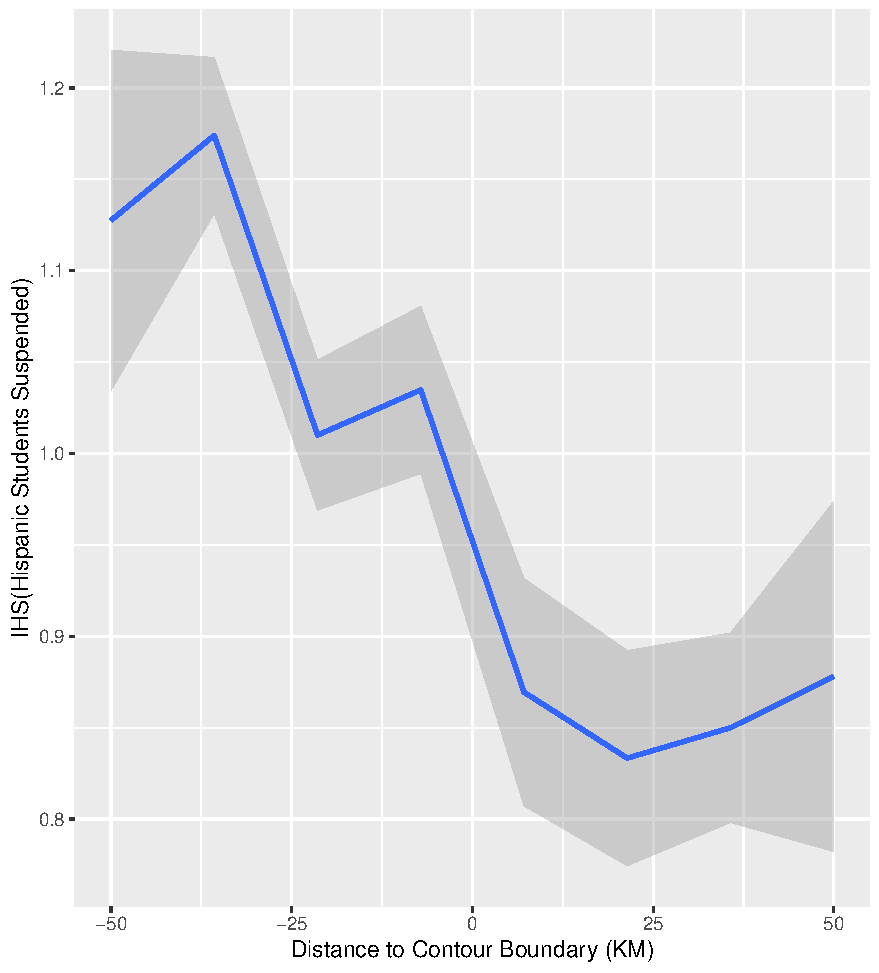
\includegraphics[width=12cm]{../../analysis/Output/graphs/hispanicsuspensions.pdf}

\textit{Notes:} The figure presents data at a school level, where a smoothed average of the inverse hyperbolic sine transformed counts of Hispanic students suspended is plotted against the distance of the school to the closest Spanish Language Television station contour boundary. Positive distances denote schools that are located within the boundary, while negative distances denote schools outside of them.
\end{figure} 

\begin{figure}[!hbtp]
\centering
\caption{Dummy for Hispanic Owned Business with Hispanic Name by Distance to Contour Boundary }\label{busnnnamefig}
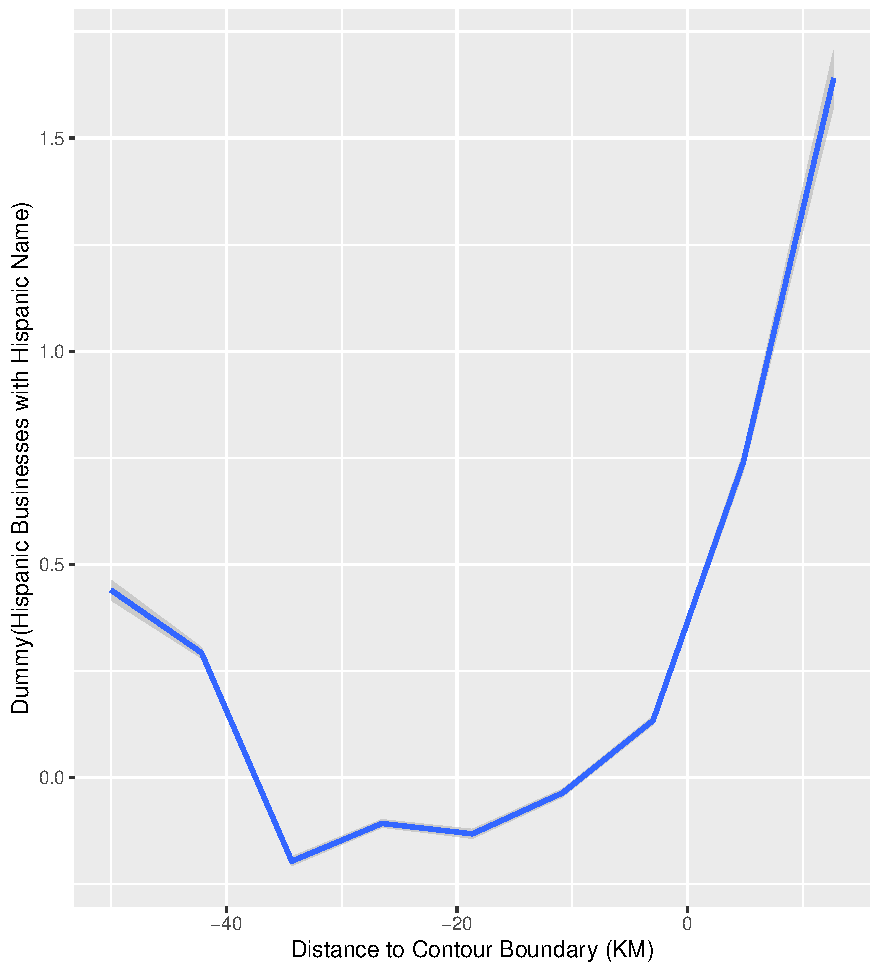
\includegraphics[width=12cm]{../../analysis/Output/graphs/hispanicbusnname.pdf}

\textit{Notes:} The figure presents data at the firm level, where a smoothed average of a residualized dummy for Hispanic businesses with Hispanic-indicating names is plotted against the distance of the school to the closest Spanish Language Television station contour boundary. Positive distances denote schools that are located within the boundary, while negative distances denote schools outside of them. Controls at the county level include log population, income, and percentage population Hispanic.
\end{figure} 

\begin{figure}[!hbtp]
\centering
\caption{IHS(\# Hispanic Donations to Trump) by Distance to Contour Boundary }\label{donationsfig}
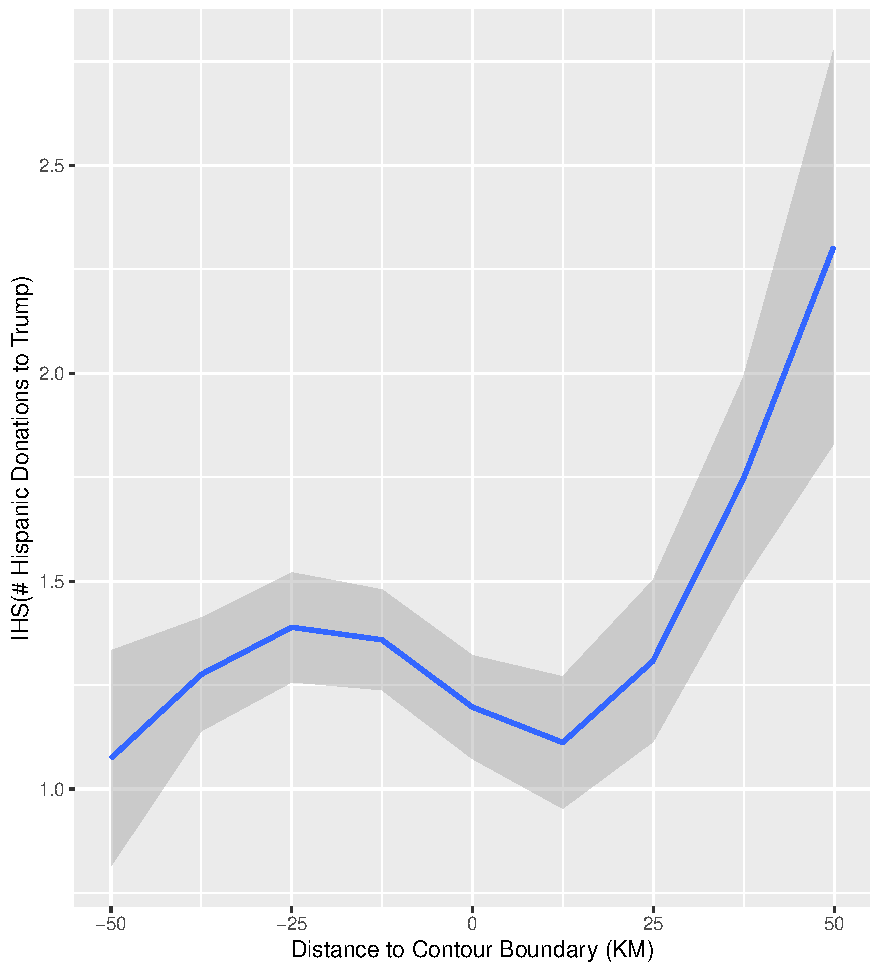
\includegraphics[width=12cm]{../../analysis/Output/graphs/hispanictrump.pdf}

\textit{Notes:} The figure presents data aggregated into squares of size approximately 4 KM$^2$, where a smoothed average of the inverse hyperbolic sine transformed counts of Hispanic campaign contributions to Trump for the 2016 election is plotted against the distance of the school to the closest Spanish Language Television station contour boundary. Positive distances denote schools that are located within the boundary, while negative distances denote schools outside of them.
\end{figure} 

\begin{figure}[!hbtp]
\centering
\caption{Coverage Map for TV Station WUVC-DT}\label{contourexamplefig}
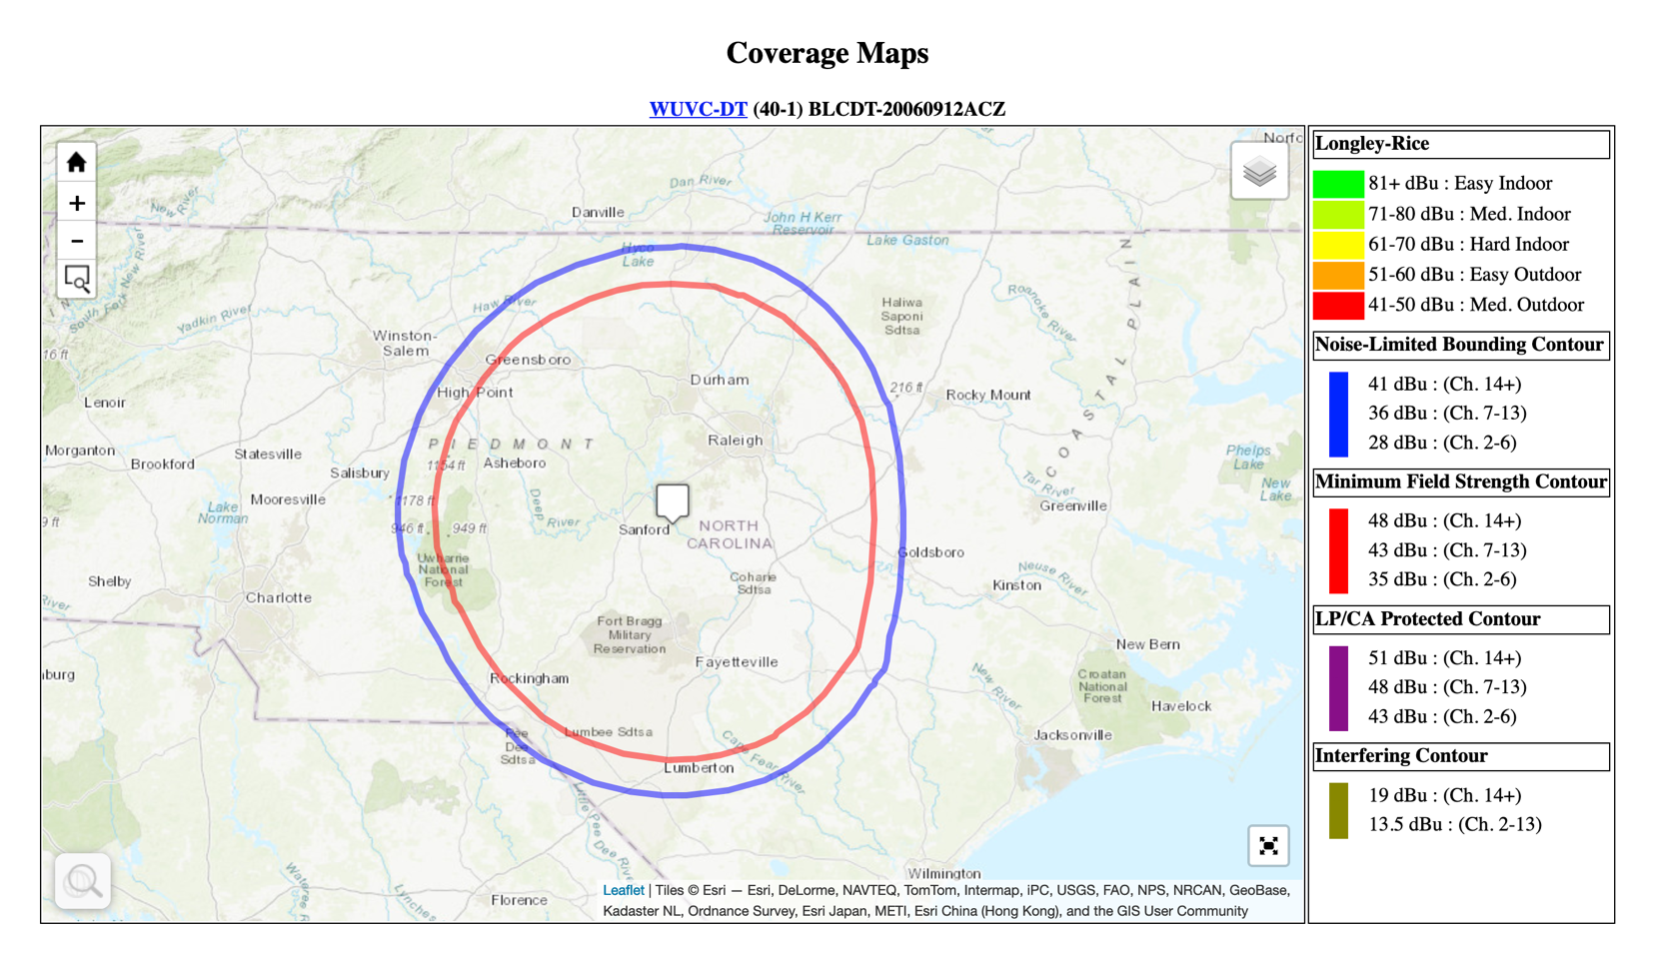
\includegraphics[width=15cm]{../../analysis/Output/img/ContourExample.png}
\end{figure} 

\begin{figure}[!hbtp]
\centering
\caption{The Coverage Contours of Spanish Language TV stations}\label{contourfig}
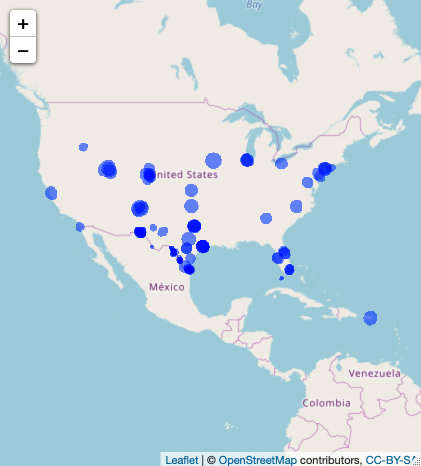
\includegraphics[width=8cm]{../../analysis/Output/img/SpanishContours.png}
\end{figure} 

\begin{figure}[!hbtp]
\centering
\caption{Map of School Districts in the US}\label{schooldistrictfig}
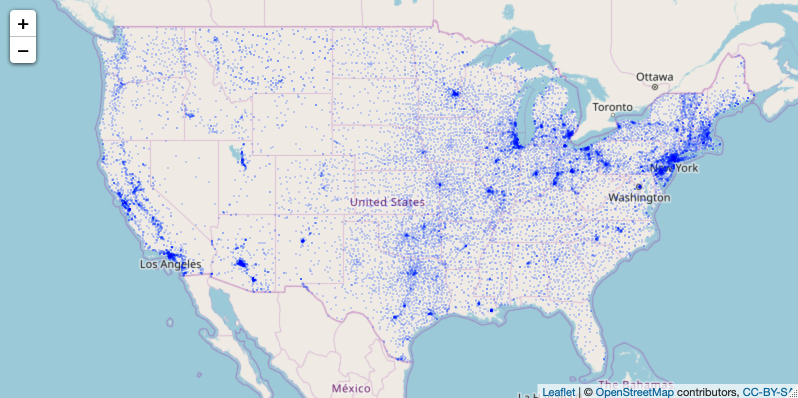
\includegraphics[width=12cm]{../../analysis/Output/img/LEAMap.png}
\end{figure} 

\clearpage
\subsection{Tables}


% Table created by stargazer v.5.2.2 by Marek Hlavac, Harvard University. E-mail: hlavac at fas.harvard.edu
% Date and time: Fri, Dec 13, 2019 - 20:45:59
\begin{table}[!htbp] \centering 
  \caption{School-District Level Summary Statistics} 
  \label{} 
\begin{tabular}{@{\extracolsep{5pt}}lccccccc} 
\\[-1.8ex]\hline 
\hline \\[-1.8ex] 
Statistic & \multicolumn{1}{c}{N} & \multicolumn{1}{c}{Mean} & \multicolumn{1}{c}{St. Dev.} & \multicolumn{1}{c}{Min} & \multicolumn{1}{c}{Pctl(25)} & \multicolumn{1}{c}{Pctl(75)} & \multicolumn{1}{c}{Max} \\ 
\hline \\[-1.8ex] 
Distance to Boundary & 17,280 & 136.855 & 146.751 & 0.000 & 15.786 & 217.567 & 806.543 \\ 
SLTV Coverage Dummy & 17,280 & 0.292 & 0.455 & 0.000 & 0.000 & 1.000 & 1.000 \\ 
\% County Hispanic & 17,280 & 7.051 & 11.950 & 0.000 & 0.668 & 6.974 & 97.216 \\ 
Log(Population) & 17,280 & 11.618 & 1.840 & 5.869 & 10.242 & 13.110 & 15.997 \\ 
Log(Income) & 17,280 & 9.428 & 0.257 & 7.976 & 9.257 & 9.593 & 10.245 \\ 
\hline \\[-1.8ex] 
\multicolumn{8}{l}{\textit{Note:} Distance to SLTV Boundary measured in KM} \\ 
\end{tabular} 
\end{table} 


% Table created by stargazer v.5.2.2 by Marek Hlavac, Harvard University. E-mail: hlavac at fas.harvard.edu
% Date and time: Fri, Dec 13, 2019 - 22:32:28
\begin{table}[!htbp] \centering 
  \caption{School Level Summary Statistics} 
  \label{} 
\begin{tabular}{@{\extracolsep{5pt}}lccccccc} 
\\[-1.8ex]\hline 
\hline \\[-1.8ex] 
Statistic & \multicolumn{1}{c}{N} & \multicolumn{1}{c}{Mean} & \multicolumn{1}{c}{St. Dev.} & \multicolumn{1}{c}{Min} & \multicolumn{1}{c}{Pctl(25)} & \multicolumn{1}{c}{Pctl(75)} & \multicolumn{1}{c}{Max} \\ 
\hline \\[-1.8ex] 
Total Students & 96,349 & 524.859 & 449.354 & 2.000 & 254.000 & 662.000 & 14,164.000 \\ 
\# Hispanic Students & 91,019 & 143.195 & 243.873 & 2.000 & 13.000 & 166.000 & 7,675.000 \\ 
Contains Grade 1 & 96,350 & 0.538 & 0.499 & 0 & 0 & 1 & 1 \\ 
Contains Grade 6 & 96,350 & 0.364 & 0.481 & 0 & 0 & 1 & 1 \\ 
Contains Grade 9 & 96,350 & 0.253 & 0.435 & 0 & 0 & 1 & 1 \\ 
Hispanic Suspension Dummy & 94,535 & 0.382 & 0.486 & 0.000 & 0.000 & 1.000 & 1.000 \\ 
Hispanic Chronic Absentees & 94,540 & 22.920 & 57.838 & 0.000 & 0.000 & 22.000 & 2,131.000 \\ 
\# Teachers & 93,934 & 35.219 & 33.892 & 1.000 & 19.000 & 44.000 & 6,031.000 \\ 
\hline \\[-1.8ex] 
\multicolumn{8}{l}{\textit{Note:} Dummies indicate whether event occurred in the school over the past year} \\ 
\end{tabular} 
\end{table} 


% Table created by stargazer v.5.2.2 by Marek Hlavac, Harvard University. E-mail: hlavac at fas.harvard.edu
% Date and time: Fri, Oct 18, 2019 - 11:56:01
\begin{table}[!htbp] \centering 
  \caption{Effect of TV on Migration, Outside Sample Distance Dummy} 
  \label{} 
\begin{tabular}{@{\extracolsep{5pt}}lcccc} 
\\[-1.8ex]\hline 
\hline \\[-1.8ex] 
 & \multicolumn{4}{c}{\textit{Dependent variable:}} \\ 
\cline{2-5} 
\\[-1.8ex] & \multicolumn{4}{c}{mig} \\ 
\\[-1.8ex] & (1) & (2) & (3) & (4)\\ 
\hline \\[-1.8ex] 
 TV & $-$138.970$^{***}$ & $-$160.743$^{***}$ & $-$164.748$^{***}$ &  \\ 
  & (50.833) & (55.860) & (58.288) &  \\ 
  & & & & \\ 
 origLogPop & 55.128$^{***}$ & 49.692$^{***}$ & 54.916$^{***}$ &  \\ 
  & (16.276) & (10.915) & (17.009) &  \\ 
  & & & & \\ 
 destLogPop & 79.360$^{**}$ & 75.183$^{**}$ & 72.917$^{**}$ &  \\ 
  & (31.339) & (29.864) & (28.813) &  \\ 
  & & & & \\ 
 origpcHisp &  & 424.714$^{***}$ & 380.709$^{***}$ &  \\ 
  &  & (149.604) & (130.054) &  \\ 
  & & & & \\ 
 destpcHisp &  & 490.885$^{***}$ & 518.338$^{***}$ &  \\ 
  &  & (145.334) & (159.358) &  \\ 
  & & & & \\ 
 origLogInc &  &  & $-$58.140 &  \\ 
  &  &  & (90.270) &  \\ 
  & & & & \\ 
 destLogInc &  &  & 29.220 &  \\ 
  &  &  & (25.991) &  \\ 
  & & & & \\ 
 origdist &  &  &  & $-$0.001 \\ 
  &  &  &  & (0.0004) \\ 
  & & & & \\ 
 destdist &  &  &  & $-$0.0001 \\ 
  &  &  &  & (0.0001) \\ 
  & & & & \\ 
 mi\_to\_county & $-$0.181$^{***}$ & $-$0.219$^{***}$ & $-$0.220$^{***}$ & $-$0.036$^{*}$ \\ 
  & (0.061) & (0.064) & (0.065) & (0.020) \\ 
  & & & & \\ 
 Constant & $-$1,446.295$^{***}$ & $-$1,395.887$^{***}$ & $-$1,156.459$^{**}$ & 135.339$^{***}$ \\ 
  & (520.832) & (457.051) & (584.710) & (24.099) \\ 
  & & & & \\ 
\hline \\[-1.8ex] 
Observations & 3,704 & 3,704 & 3,704 & 3,704 \\ 
R$^{2}$ & 0.045 & 0.064 & 0.064 & 0.002 \\ 
Adjusted R$^{2}$ & 0.044 & 0.062 & 0.062 & 0.001 \\ 
Residual Std. Error & 646.360 (df = 3699) & 640.108 (df = 3697) & 640.222 (df = 3695) & 660.720 (df = 3700) \\ 
\hline 
\hline \\[-1.8ex] 
\textit{Note:}  & \multicolumn{4}{r}{$^{*}$p$<$0.1; $^{**}$p$<$0.05; $^{***}$p$<$0.01} \\ 
\end{tabular} 
\end{table} 


% Table created by stargazer v.5.2.2 by Marek Hlavac, Harvard University. E-mail: hlavac at fas.harvard.edu
% Date and time: Fri, Oct 18, 2019 - 12:07:46
\begin{table}[!htbp] \centering 
  \caption{Effect of TV on Reverse Migration, Outside Sample Distance Dummy} 
  \label{} 
\begin{tabular}{@{\extracolsep{5pt}}lcccc} 
\\[-1.8ex]\hline 
\hline \\[-1.8ex] 
 & \multicolumn{4}{c}{\textit{Dependent variable:}} \\ 
\cline{2-5} 
\\[-1.8ex] & \multicolumn{4}{c}{revMig} \\ 
\\[-1.8ex] & (1) & (2) & (3) & (4)\\ 
\hline \\[-1.8ex] 
 TV & $-$272.468$^{***}$ & $-$302.891$^{***}$ & $-$290.716$^{***}$ &  \\ 
  & (87.512) & (96.017) & (95.484) &  \\ 
  & & & & \\ 
 origLogPop & 161.229$^{***}$ & 136.370$^{***}$ & 138.851$^{***}$ &  \\ 
  & (59.972) & (40.537) & (47.270) &  \\ 
  & & & & \\ 
 destLogPop & 148.127$^{**}$ & 144.794$^{**}$ & 156.419$^{**}$ &  \\ 
  & (63.158) & (64.019) & (66.248) &  \\ 
  & & & & \\ 
 origpcHisp &  & 894.758$^{**}$ & 890.891$^{***}$ &  \\ 
  &  & (372.920) & (323.861) &  \\ 
  & & & & \\ 
 destpcHisp &  & 683.396$^{***}$ & 574.860$^{***}$ &  \\ 
  &  & (191.365) & (178.543) &  \\ 
  & & & & \\ 
 origLogInc &  &  & $-$17.479 &  \\ 
  &  &  & (161.210) &  \\ 
  & & & & \\ 
 destLogInc &  &  & $-$121.820$^{**}$ &  \\ 
  &  &  & (62.089) &  \\ 
  & & & & \\ 
 origdist &  &  &  & $-$0.001 \\ 
  &  &  &  & (0.001) \\ 
  & & & & \\ 
 destdist &  &  &  & 0.0002 \\ 
  &  &  &  & (0.0003) \\ 
  & & & & \\ 
 mi\_to\_county & $-$0.442$^{**}$ & $-$0.504$^{***}$ & $-$0.506$^{***}$ & $-$0.083$^{*}$ \\ 
  & (0.176) & (0.172) & (0.172) & (0.050) \\ 
  & & & & \\ 
 Constant & $-$3,472.526$^{**}$ & $-$3,281.295$^{***}$ & $-$2,122.032$^{*}$ & 275.949$^{***}$ \\ 
  & (1,386.592) & (1,181.058) & (1,169.812) & (59.805) \\ 
  & & & & \\ 
\hline \\[-1.8ex] 
Observations & 1,526 & 1,526 & 1,526 & 1,526 \\ 
R$^{2}$ & 0.091 & 0.118 & 0.119 & 0.003 \\ 
Adjusted R$^{2}$ & 0.089 & 0.115 & 0.114 & 0.001 \\ 
Residual Std. Error & 1,015.579 (df = 1521) & 1,001.034 (df = 1519) & 1,001.478 (df = 1517) & 1,063.523 (df = 1522) \\ 
\hline 
\hline \\[-1.8ex] 
\textit{Note:}  & \multicolumn{4}{r}{$^{*}$p$<$0.1; $^{**}$p$<$0.05; $^{***}$p$<$0.01} \\ 
\end{tabular} 
\end{table} 


% Table created by stargazer v.5.2.2 by Marek Hlavac, Harvard University. E-mail: hlavac at fas.harvard.edu
% Date and time: Mon, Feb 03, 2020 - 17:52:42
\begin{table}[!htbp] \centering 
  \caption{Effect of TV on Hispanic Donations to Trump, 100 KM Radius} 
  \label{} 
\begin{tabular}{@{\extracolsep{-5pt}}lcccc} 
\\[-1.8ex]\hline 
\hline \\[-1.8ex] 
 & \multicolumn{4}{c}{\textit{Dependent variable:}} \\ 
\cline{2-5} 
\\[-1.8ex] & \multicolumn{4}{c}{donations} \\ 
\\[-1.8ex] & (1) & (2) & (3) & (4)\\ 
\hline \\[-1.8ex] 
 intersects & 4.650$^{***}$ & 2.941$^{***}$ & 2.506$^{**}$ & 2.175$^{**}$ \\ 
  & (1.146) & (1.079) & (1.093) & (1.072) \\ 
  & & & & \\ 
 distance & 0.015 & 0.061 & 0.062 & 0.068 \\ 
  & (0.131) & (0.123) & (0.123) & (0.120) \\ 
  & & & & \\ 
 dist2 & $-$0.00004 & $-$0.0002 & $-$0.0002 & $-$0.0002 \\ 
  & (0.001) & (0.001) & (0.001) & (0.001) \\ 
  & & & & \\ 
 logPop &  & 12.674$^{***}$ & 12.919$^{***}$ & 8.877$^{***}$ \\ 
  &  & (0.586) & (0.595) & (0.674) \\ 
  & & & & \\ 
 pcHispanic &  &  & 9.646$^{**}$ & 37.604$^{***}$ \\ 
  &  &  & (4.019) & (4.584) \\ 
  & & & & \\ 
 income &  &  &  & 0.004$^{***}$ \\ 
  &  &  &  & (0.0004) \\ 
  & & & & \\ 
 intersects:distance & 0.039 & $-$0.049 & $-$0.039 & $-$0.059 \\ 
  & (0.089) & (0.083) & (0.083) & (0.082) \\ 
  & & & & \\ 
 intersects:dist2 & 0.005$^{***}$ & 0.004$^{***}$ & 0.004$^{***}$ & 0.004$^{***}$ \\ 
  & (0.001) & (0.001) & (0.001) & (0.001) \\ 
  & & & & \\ 
 Constant & 4.818$^{*}$ & $-$125.487$^{***}$ & $-$129.366$^{***}$ & $-$139.563$^{***}$ \\ 
  & (2.672) & (6.528) & (6.721) & (6.643) \\ 
  & & & & \\ 
\hline \\[-1.8ex] 
Observations & 3,479 & 3,479 & 3,479 & 3,479 \\ 
R$^{2}$ & 0.084 & 0.193 & 0.194 & 0.226 \\ 
Adjusted R$^{2}$ & 0.083 & 0.191 & 0.192 & 0.224 \\ 
\hline 
\hline \\[-1.8ex] 
\textit{Note:}  & \multicolumn{4}{r}{$^{*}$p$<$0.1; $^{**}$p$<$0.05; $^{***}$p$<$0.01} \\ 
\end{tabular} 
\end{table} 


% Table created by stargazer v.5.2.2 by Marek Hlavac, Harvard University. E-mail: hlavac at fas.harvard.edu
% Date and time: Sun, Feb 16, 2020 - 22:18:36
\begin{table}[!htbp] \centering 
  \caption{Effect of TV on Hispanic Donations to Trump, 100 KM Radius} 
  \label{} 
\begin{tabular}{@{\extracolsep{-5pt}}lccc} 
\\[-1.8ex]\hline 
\hline \\[-1.8ex] 
 & \multicolumn{3}{c}{\textit{Dependent variable:}} \\ 
\cline{2-4} 
\\[-1.8ex] & \multicolumn{3}{c}{Dummy: Hispanic Campaign Contributors} \\ 
\\[-1.8ex] & (1) & (2) & (3)\\ 
\hline \\[-1.8ex] 
 TV Dummy & 1.767$^{***}$ & 1.342$^{*}$ & 1.191$^{*}$ \\ 
  & (0.682) & (0.690) & (0.684) \\ 
  & & & \\ 
 TV Dummy $\times$ Distance to Boundary  & $-$0.012 & $-$0.003 & $-$0.012 \\ 
  & (0.053) & (0.053) & (0.052) \\ 
  & & & \\ 
 Distance to Boundary (KM) & 0.024 & 0.025 & 0.028 \\ 
  & (0.078) & (0.077) & (0.077) \\ 
  & & & \\ 
 Log(Population) & 6.643$^{***}$ & 6.881$^{***}$ & 5.039$^{***}$ \\ 
  & (0.371) & (0.376) & (0.430) \\ 
  & & & \\ 
 County \% Hispanic &  & 9.393$^{***}$ & 22.133$^{***}$ \\ 
  &  & (2.538) & (2.923) \\ 
  & & & \\ 
 Log(Income) &  &  & 0.002$^{***}$ \\ 
  &  &  & (0.0002) \\ 
  & & & \\ 
\hline \\[-1.8ex] 
Observations & 3,479 & 3,479 & 3,479 \\ 
R$^{2}$ & 0.140 & 0.143 & 0.161 \\ 
Adjusted R$^{2}$ & 0.138 & 0.141 & 0.159 \\ 
\hline 
\hline \\[-1.8ex] 
\textit{Note:}  & \multicolumn{3}{r}{$^{*}$p$<$0.1; $^{**}$p$<$0.05; $^{***}$p$<$0.01} \\ 
\end{tabular} 
\end{table} 


% Table created by stargazer v.5.2.2 by Marek Hlavac, Harvard University. E-mail: hlavac at fas.harvard.edu
% Date and time: Mon, Feb 03, 2020 - 16:47:20
\begin{table}[!htbp] \centering 
  \caption{Effect of TV on Hispanic Donations to Clinton, 100 KM Radius} 
  \label{} 
\begin{tabular}{@{\extracolsep{-5pt}}lcccc} 
\\[-1.8ex]\hline 
\hline \\[-1.8ex] 
 & \multicolumn{4}{c}{\textit{Dependent variable:}} \\ 
\cline{2-5} 
\\[-1.8ex] & \multicolumn{4}{c}{donations} \\ 
\\[-1.8ex] & (1) & (2) & (3) & (4)\\ 
\hline \\[-1.8ex] 
 intersects & 4.863$^{*}$ & 2.698 & 0.132 & $-$0.844 \\ 
  & (2.558) & (2.489) & (2.513) & (2.481) \\ 
  & & & & \\ 
 distance & 0.0002 & 0.0001 & 0.00002 & 0.00000 \\ 
  & (0.0003) & (0.0003) & (0.0003) & (0.0003) \\ 
  & & & & \\ 
 dist2 & $-$0.000 & $-$0.000 & 0.000 & 0.000 \\ 
  & (0.000) & (0.000) & (0.000) & (0.000) \\ 
  & & & & \\ 
 logPop &  & 12.347$^{***}$ & 11.427$^{***}$ & 5.977$^{***}$ \\ 
  &  & (1.394) & (1.391) & (1.645) \\ 
  & & & & \\ 
 pcHispanic &  &  & 78.466$^{***}$ & 119.350$^{***}$ \\ 
  &  &  & (15.348) & (16.590) \\ 
  & & & & \\ 
 income &  &  &  & 0.004$^{***}$ \\ 
  &  &  &  & (0.001) \\ 
  & & & & \\ 
 intersects:distance & $-$0.0001 & $-$0.0001 & $-$0.0001 & $-$0.0001 \\ 
  & (0.0002) & (0.0002) & (0.0001) & (0.0001) \\ 
  & & & & \\ 
 intersects:dist2 & 0.000$^{*}$ & 0.000 & 0.000$^{*}$ & 0.000$^{*}$ \\ 
  & (0.000) & (0.000) & (0.000) & (0.000) \\ 
  & & & & \\ 
 Constant & 3.994 & $-$136.034$^{***}$ & $-$126.548$^{***}$ & $-$122.380$^{***}$ \\ 
  & (6.612) & (17.060) & (16.979) & (16.743) \\ 
  & & & & \\ 
\hline \\[-1.8ex] 
Observations & 1,164 & 1,164 & 1,164 & 1,164 \\ 
R$^{2}$ & 0.032 & 0.093 & 0.113 & 0.140 \\ 
Adjusted R$^{2}$ & 0.028 & 0.088 & 0.108 & 0.134 \\ 
\hline 
\hline \\[-1.8ex] 
\textit{Note:}  & \multicolumn{4}{r}{$^{*}$p$<$0.1; $^{**}$p$<$0.05; $^{***}$p$<$0.01} \\ 
\end{tabular} 
\end{table} 


% Table created by stargazer v.5.2.2 by Marek Hlavac, Harvard University. E-mail: hlavac at fas.harvard.edu
% Date and time: Mon, Feb 03, 2020 - 17:59:07
\begin{table}[!htbp] \centering 
  \caption{Effect of TV on Hispanic Donations to Clinton, 100 KM Radius} 
  \label{} 
\begin{tabular}{@{\extracolsep{-5pt}}lccc} 
\\[-1.8ex]\hline 
\hline \\[-1.8ex] 
 & \multicolumn{3}{c}{\textit{Dependent variable:}} \\ 
\cline{2-4} 
\\[-1.8ex] & \multicolumn{3}{c}{donations\_d} \\ 
\\[-1.8ex] & (1) & (2) & (3)\\ 
\hline \\[-1.8ex] 
 intersects & 0.153 & 0.049 & 0.014 \\ 
  & (0.181) & (0.183) & (0.182) \\ 
  & & & \\ 
 distance & 0.009 & 0.009 & 0.009 \\ 
  & (0.021) & (0.021) & (0.020) \\ 
  & & & \\ 
 dist2 & $-$0.00002 & $-$0.00001 & $-$0.00000 \\ 
  & (0.0002) & (0.0002) & (0.0002) \\ 
  & & & \\ 
 logPop & 1.274$^{***}$ & 1.333$^{***}$ & 0.900$^{***}$ \\ 
  & (0.098) & (0.100) & (0.114) \\ 
  & & & \\ 
 pcHispanic &  & 2.305$^{***}$ & 5.296$^{***}$ \\ 
  &  & (0.673) & (0.777) \\ 
  & & & \\ 
 income &  &  & 0.0005$^{***}$ \\ 
  &  &  & (0.0001) \\ 
  & & & \\ 
 intersects:distance & 0.003 & 0.005 & 0.003 \\ 
  & (0.014) & (0.014) & (0.014) \\ 
  & & & \\ 
 intersects:dist2 & 0.0004$^{*}$ & 0.0004$^{*}$ & 0.0004$^{*}$ \\ 
  & (0.0002) & (0.0002) & (0.0002) \\ 
  & & & \\ 
 Constant & $-$12.861$^{***}$ & $-$13.788$^{***}$ & $-$14.879$^{***}$ \\ 
  & (1.094) & (1.125) & (1.126) \\ 
  & & & \\ 
\hline \\[-1.8ex] 
Observations & 3,479 & 3,479 & 3,479 \\ 
R$^{2}$ & 0.084 & 0.087 & 0.102 \\ 
Adjusted R$^{2}$ & 0.082 & 0.085 & 0.100 \\ 
\hline 
\hline \\[-1.8ex] 
\textit{Note:}  & \multicolumn{3}{r}{$^{*}$p$<$0.1; $^{**}$p$<$0.05; $^{***}$p$<$0.01} \\ 
\end{tabular} 
\end{table} 


\begin{table}[!h]
	\centering
	\captionsetup{skip=1.5pt}
	\caption{Robustness of Influence of Spanish Language Television on Hispanic Business Ownership} \label{firm_busn}
	\scalebox{.8}{
		\begin{threeparttable}
			\begin{tabular}{lcccccccccc}
				\hline\hline\addlinespace
				 & \multicolumn{4}{c}{\textit{IHS(\# Hispanic Owned Businesses)}}\\
				&  (1) & (2) & (3) & (4) \\
                                \hline\addlinespace
 TV Dummy & 0.261$^{***}$ & 0.122$^{***}$ & 0.112$^{***}$ & 0.132$^{***}$ \\ 
  & (0.014) & (0.014) & (0.014) & (0.015) \\ 
 TV Dummy $\times$ Distance to Boundary & 0.010$^{***}$ & 0.007$^{***}$ & 0.007$^{***}$ & 0.007$^{***}$ \\ 
  & (0.001) & (0.001) & (0.001) & (0.001) \\ 
 Distance to Boundary (meters) & 0.006$^{***}$ & 0.009$^{***}$ & 0.010$^{***}$ & 0.011$^{***}$ \\ 
  & (0.001) & (0.001) & (0.001) & (0.001) \\ 
 Log(Population) &  & 0.412$^{***}$ & 0.388$^{***}$ & 0.342$^{***}$ \\ 
  &  & (0.011) & (0.012) & (0.014) \\ 
 County \% Hispanic &  &  & 1.261$^{***}$ & 1.414$^{***}$ \\ 
  &  &  & (0.133) & (0.136) \\ 
 Log(Income) &  &  &  & 0.391$^{***}$ \\ 
  &  &  &  & (0.070) \\ 
Observations & 23,853 & 23,853 & 23,853 & 23,853 \\ 
				\addlinespace\hline\hline
			\end{tabular}
			\begin{tablenotes}[flushleft]
				\item \textit{Notes:} The table presents coefficient estimates from regressions at aggregated into grids of size approximately 4 KM$^2$, only keeping grid points within 100 KM of a contour boundary. The dependent variable is the inverse hyperbolic sine transformed counts of Hispanic owned firms within the grid. The key dependent variable of interest is the TV Dummy, which tracks whether the school is within a coverage contour boundary for a Spanish language television station. This is interacted with the distance to the boundary. Controls are at the county level Standard errors are given in parentheses. *, **, and *** denote statistical significance at the 10\%, 5\%, and 1\% levels, respectively.
			\end{tablenotes}
		\end{threeparttable}
	}
\end{table}
\begin{table}[!h]
	\centering
	\captionsetup{skip=1.5pt}
	\caption{Robustness of Influence of Spanish Language Television on Hispanic Business Ownership} \label{firm_busn}
	\scalebox{.8}{
		\begin{threeparttable}
			\begin{tabular}{lcccccccccc}
				\hline\hline\addlinespace
				 & \multicolumn{6}{c}{\textit{IHS(\# Hispanic Owned Businesses)}}\\
				&  (1) & (2) & (3) & (4) & (5) & (6) \\
                                \hline\addlinespace
 TV Dummy & 0.839$^{***}$ & 0.638$^{***}$ & 0.637$^{***}$ & 0.769$^{***}$ & 0.849$^{***}$ & 0.775$^{***}$ \\ 
  & (0.052) & (0.066) & (0.066) & (0.071) & (0.077) & (0.071) \\ 
 TV Dummy $\times$ Distance to Boundary & 0.008$^{***}$ & 0.002 & 0.002 & 0.0002 & $-$0.0002 & 0.0002 \\ 
  & (0.002) & (0.002) & (0.002) & (0.002) & (0.002) & (0.002) \\ 
 Distance to Boundary (meters) & 0.010$^{**}$ & 0.021$^{***}$ & 0.021$^{***}$ & 0.031$^{***}$ & 0.035$^{***}$ & 0.031$^{***}$ \\ 
  & (0.004) & (0.004) & (0.005) & (0.005) & (0.005) & (0.005) \\ 
 Log(Population) &  & 0.957$^{***}$ & 0.979$^{***}$ & 0.702$^{***}$ & 0.761$^{***}$ & 0.701$^{***}$ \\ 
  &  & (0.052) & (0.070) & (0.074) & (0.081) & (0.074) \\ 
 County \% Hispanic &  &  & $-$0.151 & 1.428$^{***}$ & 1.514$^{***}$ & 1.434$^{***}$ \\ 
  &  &  & (0.312) & (0.367) & (0.388) & (0.368) \\ 
 Log(Income) &  &  &  & 2.350$^{***}$ & 2.534$^{***}$ & 2.356$^{***}$ \\ 
  &  &  &  & (0.319) & (0.344) & (0.320) \\ 
Observations & 23,853 & 23,853 & 23,853 & 23,853 & 23,853 & 23,853 \\ 
				\hline\hline\addlinespace
				Only Hispanic Owners & No & No & No & No & Yes & No \\
				Only Non-Hispanic Owners & No & No & No & No & No & Yes \\
				\addlinespace\hline\hline
			\end{tabular}
			\begin{tablenotes}[flushleft]
				\item \textit{Notes:} The table presents coefficient estimates from logit regressions at aggregated into grids of size approximately 4 KM$^2$, only keeping grid points within 100 KM of a contour boundary. The dependent variable is a dummy for whether there is a firm with a Hispanic name within the grid. The key dependent variable of interest is the TV Dummy, which tracks whether the school is within a coverage contour boundary for a Spanish language television station. This is interacted with the distance to the boundary. Controls are at the county level. Standard errors are given in parentheses. *, **, and *** denote statistical significance at the 10\%, 5\%, and 1\% levels, respectively.
			\end{tablenotes}
		\end{threeparttable}
	}
\end{table}
\begin{table}[!h]
	\centering
	\captionsetup{skip=1.5pt}
	\caption{Robustness of Influence of Spanish Language Television on Hispanic Owned Businesses with Hispanic Names} \label{firm_robust}
	\scalebox{.8}{
		\begin{threeparttable}
			\begin{tabular}{lcccccccccc}
				\hline\hline\addlinespace
				 & \multicolumn{8}{c}{\textit{Hispanic Owned and Named Business Dummy}}\\
				&  (1) & (2) & (3) & (4) & (5) & (6) & (7) & (8) \\
                                \hline\addlinespace
 TV Dummy & 0.849$^{***}$ & 1.071$^{***}$ & 0.305$^{***}$ & .8677$^{***}$ & 0.927$^{***}$ & 0.596$^{***}$ & 0.624$^{***}$ & 1.144$^{***}$ \\ 
  & (0.077) & (0.115) & (0.078) & (0.079) & (0.098) & (0.118) & (0.078) & (0.076) \\ 
 TV Dummy $\times$ Distance to Boundary  & $-$0.0002 & $-$0.008 & $-$0.003 & $-$0.001 & $-$0.002 & 0.042$^{***}$ & 0.001 & $-$0.001 \\ 
  & (0.002) & (0.007) & (0.002) & (0.002) & (0.004) & (0.010) & (0.002) & (0.002) \\ 
 Distance to Boundary (meters) & 0.035$^{***}$ & 0.123$^{***}$ & 0.013$^{***}$ & 0.036$^{***}$ & 0.049$^{***}$ & $-$0.097$^{***}$ & 0.026$^{***}$ & 0.042$^{***}$ \\ 
  & (0.005) & (0.021) & (0.005) & (0.005) & (0.012) & (0.035) & (0.005) & (0.006) \\ 
 Total Businesses &  &  & 0.023$^{***}$ &  &  &  &  &  \\ 
  &  &  & (0.001) &  &  &  &  &  \\ 
\hline \\[-1.8ex] 
Observations & 23,853 & 23,853 & 23,853 & 23,853 & 20,404 & 14,386 & 10,598 & 95,373 \\ 				\hline\hline\addlinespace
County Controls & Yes & Yes & Yes & Yes & Yes & Yes & Yes & Yes \\
Distance Cutoff (KM) & 100 & 100 & 100 & 100 & 50 &25 & 100 &100 \\
Grid Size (KM$^2$) & 4 & 4 & 4 & 4 &4 & 4 & 9 & 1\\ 
Distance$^2$ & No & Yes & No & No & No & No & No & No \\
No Food Names & No & No & No & Yes & No & No & No & No \\
				\addlinespace\hline\hline
			\end{tabular}
			\begin{tablenotes}[flushleft]
				\item \textit{Notes:} The table presents coefficient estimates from logit regressions at aggregated into grids, only keeping grid points within a certain cutoff of a contour boundary. The dependent variable is a dummy for whether there is a firm with a Hispanic name owned by a Hispanic person within the grid. Column (1) is the same specification as Table \ref{firm_name} Column (5). The key independent variable of interest is the TV Dummy, which tracks whether the school is within a coverage contour boundary for a Spanish language television station. This is interacted with the distance to the boundary. Controls are at the county level, and include log population, log income, and percentage of county that is Hispanic. Total Businesses is the total number of businesses in the grid, while No Food Names removes references to various Hispanic foods as part of the criterion for selection of Hispanic business names. Various distance cut-offs, grid sizes, as well as the interaction with distance squared are presented. Standard errors are given in parentheses. *, **, and *** denote statistical significance at the 10\%, 5\%, and 1\% levels, respectively.
			\end{tablenotes}
		\end{threeparttable}
	}
\end{table}
\begin{table}[!h]
	\centering
	\captionsetup{skip=1.5pt}
	\caption{Spatial Robustness of Influence of Spanish Language Television on Hispanic Firm Ownership} \label{firm_spatial}
	\scalebox{.8}{
		\begin{threeparttable}
			\begin{tabular}{lcccccccccc}
				\hline\hline\addlinespace
				 & \multicolumn{3}{c}{\textit{IHS(\# Hispanic Owned Firms)}}\\
				&  (1) & (2) & (3) \\
                                \hline\addlinespace
 TV Dummy & 0.122$^{***}$ & 0.022$^{***}$ & 0.126$^{***}$ \\ 
  & (0.014) & (0.006) & (0.036) \\ 
\hline\hline\addlinespace
Observations & 23,853 & 23,853 & 23,853 \\ 
Log Likelihood &  & $-$38,404 & $-$38,440 \\ 
$\sigma^{2}$ &  & 1.168 & 1.170 \\ 
Akaike Inf. Crit. &  & 76,821 & 76,894 \\ 
Wald Test (df = 1) &  & 65,139$^{***}$ & 63,913$^{***}$ \\ 
LR Test (df = 1) &  & 24,759$^{***}$ & 24,687$^{***}$ \\ 
\hline \addlinespace
                                County Controls & Yes & Yes  & Yes \\
                                Model & OLS & SAR Lag & SAR Error \\
				\addlinespace\hline\hline
			\end{tabular}
			\begin{tablenotes}[flushleft]
				\item \textit{Notes:} The table presents coefficient estimates from regressions at aggregated into grids of size approximately 4 KM$^2$, only keeping grid points within 100 KM of a contour boundary. The dependent variable is the inverse hyperbolic sine transformed counts of Hispanic owned firms in the grid. The key dependent variable of interest is the TV Dummy, which tracks whether the school is within a coverage contour boundary for a Spanish language television station. This is interacted with the distance to the boundary. County controls include log population. Additionally controlling for log income and percentage county Hispanic for the county which the grid is in yields similar coefficients, although standard errors cannot be estimated due to computational limitations. The SAR Lag model is a spatial autoregressive lag model and the SAR Error model is a spatial autoregressive error model, both with weight matrices based on 4 nearest neighbours. Standard errors are given in parentheses. *, **, and *** denote statistical significance at the 10\%, 5\%, and 1\% levels, respectively.
			\end{tablenotes}
		\end{threeparttable}
	}
\end{table}

%
% Table created by stargazer v.5.2.2 by Marek Hlavac, Harvard University. E-mail: hlavac at fas.harvard.edu
% Date and time: Thu, Jan 23, 2020 - 17:05:20
\begin{table}[!htbp] \centering 
  \caption{Effect of TV on IHS(Hispanic Out of School Suspension)} 
  \label{} 
\begin{tabular}{@{\extracolsep{-2pt}}lcccc} 
\\[-1.8ex]\hline 
\hline \\[-1.8ex] 
 & \multicolumn{4}{c}{\textit{Dependent variable:}} \\ 
\cline{2-5} 
\\[-1.8ex] & \multicolumn{4}{c}{IHS(\# Hispanic Out of School Suspension)} \\ 
\\[-1.8ex] & (1) & (2) & (3) & (4)\\ 
\hline \\[-1.8ex] 
 TV Dummy & 0.189$^{***}$ & 0.053$^{***}$ & 0.072$^{***}$ & 0.033$^{**}$ \\ 
  & (0.020) & (0.016) & (0.016) & (0.016) \\ 
  & & & & \\ 
 TV Dummy $\times$ Distance to Boundary & 0.013$^{***}$ & 0.003$^{***}$ & 0.005$^{***}$ & 0.005$^{***}$ \\ 
  & (0.001) & (0.001) & (0.001) & (0.001) \\ 
  & & & & \\ 
 TV Dummy $\times$ Distance2 & $-$0.0002$^{***}$ & $-$0.00001 & $-$0.00003 & $-$0.00002 \\ 
  & (0.00002) & (0.00002) & (0.00002) & (0.00002) \\ 
  & & & & \\ 
 Distance to Boundary (meters) & $-$0.006$^{***}$ & $-$0.004$^{***}$ & $-$0.004$^{***}$ & $-$0.006$^{***}$ \\ 
  & (0.001) & (0.001) & (0.001) & (0.001) \\ 
  & & & & \\ 
 Distance2 & 0.00005$^{***}$ & 0.00004$^{***}$ & 0.00004$^{***}$ & 0.00005$^{***}$ \\ 
  & (0.00001) & (0.00001) & (0.00001) & (0.00001) \\ 
  & & & & \\ 
 \% County Hispanic & 1.356$^{***}$ & $-$0.300$^{***}$ & $-$0.326$^{***}$ & $-$0.550$^{***}$ \\ 
  & (0.044) & (0.041) & (0.040) & (0.042) \\ 
  & & & & \\ 
 Log(Population) & $-$0.218$^{***}$ & $-$0.430$^{***}$ & $-$0.371$^{***}$ & $-$0.575$^{***}$ \\ 
  & (0.023) & (0.019) & (0.019) & (0.022) \\ 
  & & & & \\ 
 \# Teachers at School &  & 0.007$^{***}$ & 0.005$^{***}$ & 0.006$^{***}$ \\ 
  &  & (0.0003) & (0.0003) & (0.0003) \\ 
  & & & & \\ 
 \# Hispanic Students &  & 0.002$^{***}$ & 0.002$^{***}$ & 0.002$^{***}$ \\ 
  &  & (0.00003) & (0.00003) & (0.00003) \\ 
  & & & & \\ 
 Total Students &  & 0.0001$^{***}$ & 0.0001$^{***}$ & 0.00004$^{*}$ \\ 
  &  & (0.00002) & (0.00002) & (0.00002) \\ 
  & & & & \\ 
 Contains Grade 1 &  &  & $-$0.545$^{***}$ & $-$0.558$^{***}$ \\ 
  &  &  & (0.011) & (0.011) \\ 
  & & & & \\ 
 Contains Grade 6 &  &  & 0.202$^{***}$ & 0.192$^{***}$ \\ 
  &  &  & (0.010) & (0.010) \\ 
  & & & & \\ 
 Contains Grade 9 &  &  & 0.011 & 0.010 \\ 
  &  &  & (0.013) & (0.013) \\ 
  & & & & \\ 
 Log(Income) &  &  &  & 0.067$^{***}$ \\ 
  &  &  &  & (0.004) \\ 
  & & & & \\ 
\hline \\[-1.8ex] 
Observations & 45,947 & 45,947 & 45,947 & 45,947 \\ 
R$^{2}$ & 0.067 & 0.344 & 0.400 & 0.404 \\ 
Adjusted R$^{2}$ & 0.067 & 0.344 & 0.400 & 0.403 \\ 
\hline 
\hline \\[-1.8ex] 
\textit{Note:}  & \multicolumn{4}{r}{$^{*}$p$<$0.1; $^{**}$p$<$0.05; $^{***}$p$<$0.01} \\ 
\end{tabular} 
\end{table} 

%
% Table created by stargazer v.5.2.2 by Marek Hlavac, Harvard University. E-mail: hlavac at fas.harvard.edu
% Date and time: Sun, Feb 02, 2020 - 15:39:31
\begin{table}[!htbp] \centering 
  \caption{Effect of TV on IHS(Hispanic \# Harassment Victims)} 
  \label{} 
\begin{tabular}{@{\extracolsep{-2pt}}lcccc} 
\\[-1.8ex]\hline 
\hline \\[-1.8ex] 
 & \multicolumn{4}{c}{\textit{Dependent variable:}} \\ 
\cline{2-5} 
\\[-1.8ex] & \multicolumn{4}{c}{IHS(\# Hispanic Victims of Harassment)} \\ 
\\[-1.8ex] & (1) & (2) & (3) & (4)\\ 
\hline \\[-1.8ex] 
 TV Dummy & 0.021$^{***}$ & 0.018$^{***}$ & 0.018$^{***}$ & 0.022$^{***}$ \\ 
  & (0.004) & (0.004) & (0.004) & (0.004) \\ 
  & & & & \\ 
 TV Dummy $\times$ Distance to Boundary & $-$0.001$^{*}$ & $-$0.001$^{**}$ & $-$0.001$^{**}$ & $-$0.001$^{**}$ \\ 
  & (0.0003) & (0.0003) & (0.0003) & (0.0003) \\ 
  & & & & \\ 
 TV Dummy $\times$ Distance2 & 0.00000 & 0.00000 & 0.00000 & 0.00000 \\ 
  & (0.00000) & (0.00000) & (0.00000) & (0.00000) \\ 
  & & & & \\ 
 Distance to Boundary (meters) & $-$0.0004$^{**}$ & $-$0.0004$^{*}$ & $-$0.0004$^{*}$ & $-$0.0003 \\ 
  & (0.0002) & (0.0002) & (0.0002) & (0.0002) \\ 
  & & & & \\ 
 Distance2 & 0.00000$^{*}$ & 0.00000$^{*}$ & 0.00000$^{*}$ & 0.00000 \\ 
  & (0.00000) & (0.00000) & (0.00000) & (0.00000) \\ 
  & & & & \\ 
 \% County Hispanic & 0.023$^{**}$ & $-$0.005 & $-$0.005 & 0.015 \\ 
  & (0.010) & (0.011) & (0.011) & (0.011) \\ 
  & & & & \\ 
 Log(Population) & 0.060$^{***}$ & 0.048$^{***}$ & 0.051$^{***}$ & 0.070$^{***}$ \\ 
  & (0.005) & (0.005) & (0.005) & (0.006) \\ 
  & & & & \\ 
 \# Teachers at School &  & 0.001$^{***}$ & 0.001$^{***}$ & 0.001$^{***}$ \\ 
  &  & (0.0001) & (0.0001) & (0.0001) \\ 
  & & & & \\ 
 \# Hispanic Students &  & 0.00003$^{***}$ & 0.00004$^{***}$ & 0.00004$^{***}$ \\ 
  &  & (0.00001) & (0.00001) & (0.00001) \\ 
  & & & & \\ 
 Total Students &  & $-$0.00002$^{***}$ & $-$0.00003$^{***}$ & $-$0.00002$^{***}$ \\ 
  &  & (0.00001) & (0.00001) & (0.00001) \\ 
  & & & & \\ 
 Contains Grade 1 &  &  & $-$0.037$^{***}$ & $-$0.036$^{***}$ \\ 
  &  &  & (0.003) & (0.003) \\ 
  & & & & \\ 
 Contains Grade 6 &  &  & 0.027$^{***}$ & 0.028$^{***}$ \\ 
  &  &  & (0.003) & (0.003) \\ 
  & & & & \\ 
 Contains Grade 9 &  &  & $-$0.009$^{**}$ & $-$0.009$^{**}$ \\ 
  &  &  & (0.004) & (0.004) \\ 
  & & & & \\ 
 Log(Income) &  &  &  & $-$0.006$^{***}$ \\ 
  &  &  &  & (0.001) \\ 
  & & & & \\ 
\hline \\[-1.8ex] 
Observations & 45,894 & 45,894 & 45,894 & 45,894 \\ 
R$^{2}$ & 0.008 & 0.014 & 0.021 & 0.022 \\ 
Adjusted R$^{2}$ & 0.007 & 0.014 & 0.021 & 0.022 \\ 
\hline 
\hline \\[-1.8ex] 
\textit{Note:}  & \multicolumn{4}{r}{$^{*}$p$<$0.1; $^{**}$p$<$0.05; $^{***}$p$<$0.01} \\ 
\end{tabular} 
\end{table} 

%
% Table created by stargazer v.5.2.2 by Marek Hlavac, Harvard University. E-mail: hlavac at fas.harvard.edu
% Date and time: Sun, Feb 02, 2020 - 15:48:38
\begin{table}[!htbp] \centering 
  \caption{Effect of TV on IHS(APs Taken)} 
  \label{} 
\begin{tabular}{@{\extracolsep{-2pt}}lcccc} 
\\[-1.8ex]\hline 
\hline \\[-1.8ex] 
 & \multicolumn{4}{c}{\textit{Dependent variable:}} \\ 
\cline{2-5} 
\\[-1.8ex] & \multicolumn{4}{c}{IHS(APs Taken by Hispanic Students)} \\ 
\\[-1.8ex] & (1) & (2) & (3) & (4)\\ 
\hline \\[-1.8ex] 
 TV Dummy & 0.307$^{***}$ & 0.223$^{***}$ & 0.232$^{***}$ & 0.166$^{***}$ \\ 
  & (0.065) & (0.048) & (0.047) & (0.047) \\ 
  & & & & \\ 
 TV Dummy $\times$ Distance to Boundary & 0.016$^{***}$ & 0.007$^{*}$ & 0.006$^{*}$ & 0.008$^{**}$ \\ 
  & (0.005) & (0.004) & (0.004) & (0.004) \\ 
  & & & & \\ 
 TV Dummy $\times$ Distance2 & $-$0.0001$^{*}$ & $-$0.00002 & $-$0.00002 & $-$0.00002 \\ 
  & (0.0001) & (0.0001) & (0.0001) & (0.0001) \\ 
  & & & & \\ 
 Distance to Boundary (meters) & $-$0.0002 & 0.003 & 0.003 & $-$0.002 \\ 
  & (0.004) & (0.003) & (0.003) & (0.003) \\ 
  & & & & \\ 
 Distance2 & $-$0.00005 & $-$0.0001$^{*}$ & $-$0.0001$^{**}$ & $-$0.00002 \\ 
  & (0.00005) & (0.00003) & (0.00003) & (0.00003) \\ 
  & & & & \\ 
 \% County Hispanic & 2.358$^{***}$ & 1.012$^{***}$ & 1.042$^{***}$ & 0.764$^{***}$ \\ 
  & (0.124) & (0.108) & (0.107) & (0.111) \\ 
  & & & & \\ 
 Log(Population) & $-$0.319$^{***}$ & $-$0.033 & $-$0.044 & $-$0.266$^{***}$ \\ 
  & (0.072) & (0.054) & (0.054) & (0.060) \\ 
  & & & & \\ 
 \# Teachers at School &  & $-$0.005$^{***}$ & $-$0.005$^{***}$ & $-$0.005$^{***}$ \\ 
  &  & (0.0005) & (0.0005) & (0.0005) \\ 
  & & & & \\ 
 \# Hispanic Students &  & 0.001$^{***}$ & 0.001$^{***}$ & 0.001$^{***}$ \\ 
  &  & (0.00003) & (0.00003) & (0.00003) \\ 
  & & & & \\ 
 Total Students &  & 0.0003$^{***}$ & 0.0003$^{***}$ & 0.0003$^{***}$ \\ 
  &  & (0.00003) & (0.00003) & (0.00003) \\ 
  & & & & \\ 
 Contains Grade 1 &  &  & $-$0.532$^{***}$ & $-$0.564$^{***}$ \\ 
  &  &  & (0.126) & (0.124) \\ 
  & & & & \\ 
 Contains Grade 6 &  &  & $-$0.170$^{**}$ & $-$0.225$^{***}$ \\ 
  &  &  & (0.068) & (0.067) \\ 
  & & & & \\ 
 Contains Grade 9 &  &  & 0.153$^{*}$ & 0.189$^{**}$ \\ 
  &  &  & (0.079) & (0.078) \\ 
  & & & & \\ 
 Log(Income) &  &  &  & 0.098$^{***}$ \\ 
  &  &  &  & (0.012) \\ 
  & & & & \\ 
\hline \\[-1.8ex] 
Observations & 2,342 & 2,342 & 2,342 & 2,342 \\ 
R$^{2}$ & 0.311 & 0.626 & 0.634 & 0.644 \\ 
Adjusted R$^{2}$ & 0.309 & 0.624 & 0.632 & 0.642 \\ 
\hline 
\hline \\[-1.8ex] 
\textit{Note:}  & \multicolumn{4}{r}{$^{*}$p$<$0.1; $^{**}$p$<$0.05; $^{***}$p$<$0.01} \\ 
\end{tabular} 
\end{table} 

%
% Table created by stargazer v.5.2.2 by Marek Hlavac, Harvard University. E-mail: hlavac at fas.harvard.edu
% Date and time: Sun, Feb 02, 2020 - 15:48:41
\begin{table}[!htbp] \centering 
  \caption{Effect of TV on IHS(APs Passed)} 
  \label{} 
\begin{tabular}{@{\extracolsep{-2pt}}lcccc} 
\\[-1.8ex]\hline 
\hline \\[-1.8ex] 
 & \multicolumn{4}{c}{\textit{Dependent variable:}} \\ 
\cline{2-5} 
\\[-1.8ex] & \multicolumn{4}{c}{IHS(APs Passed by Hispanic Students)} \\ 
\\[-1.8ex] & (1) & (2) & (3) & (4)\\ 
\hline \\[-1.8ex] 
 TV Dummy & 0.305$^{***}$ & 0.242$^{***}$ & 0.251$^{***}$ & 0.184$^{***}$ \\ 
  & (0.061) & (0.052) & (0.052) & (0.052) \\ 
  & & & & \\ 
 TV Dummy $\times$ Distance to Boundary & 0.005 & $-$0.003 & $-$0.004 & $-$0.002 \\ 
  & (0.005) & (0.004) & (0.004) & (0.004) \\ 
  & & & & \\ 
 TV Dummy $\times$ Distance2 & $-$0.00004 & 0.00005 & 0.0001 & 0.00005 \\ 
  & (0.0001) & (0.0001) & (0.0001) & (0.0001) \\ 
  & & & & \\ 
 Distance to Boundary (meters) & 0.005 & 0.007$^{**}$ & 0.008$^{**}$ & 0.003 \\ 
  & (0.004) & (0.003) & (0.003) & (0.003) \\ 
  & & & & \\ 
 Distance2 & $-$0.0001$^{*}$ & $-$0.0001$^{***}$ & $-$0.0001$^{***}$ & $-$0.0001 \\ 
  & (0.00004) & (0.00004) & (0.00004) & (0.00004) \\ 
  & & & & \\ 
 \% County Hispanic & 1.902$^{***}$ & 1.306$^{***}$ & 1.332$^{***}$ & 1.053$^{***}$ \\ 
  & (0.118) & (0.117) & (0.117) & (0.122) \\ 
  & & & & \\ 
 Log(Population) & 0.144$^{**}$ & 0.383$^{***}$ & 0.377$^{***}$ & 0.153$^{**}$ \\ 
  & (0.069) & (0.058) & (0.059) & (0.065) \\ 
  & & & & \\ 
 \# Teachers at School &  & $-$0.005$^{***}$ & $-$0.005$^{***}$ & $-$0.004$^{***}$ \\ 
  &  & (0.001) & (0.001) & (0.001) \\ 
  & & & & \\ 
 \# Hispanic Students &  & 0.001$^{***}$ & 0.001$^{***}$ & 0.001$^{***}$ \\ 
  &  & (0.00004) & (0.00004) & (0.00004) \\ 
  & & & & \\ 
 Total Students &  & 0.0004$^{***}$ & 0.0004$^{***}$ & 0.0004$^{***}$ \\ 
  &  & (0.00003) & (0.00003) & (0.00003) \\ 
  & & & & \\ 
 Contains Grade 1 &  &  & $-$0.216 & $-$0.248$^{*}$ \\ 
  &  &  & (0.137) & (0.136) \\ 
  & & & & \\ 
 Contains Grade 6 &  &  & $-$0.186$^{**}$ & $-$0.241$^{***}$ \\ 
  &  &  & (0.074) & (0.074) \\ 
  & & & & \\ 
 Contains Grade 9 &  &  & 0.133 & 0.169$^{**}$ \\ 
  &  &  & (0.086) & (0.085) \\ 
  & & & & \\ 
 Log(Income) &  &  &  & 0.098$^{***}$ \\ 
  &  &  &  & (0.013) \\ 
  & & & & \\ 
\hline \\[-1.8ex] 
Observations & 2,342 & 2,342 & 2,342 & 2,342 \\ 
R$^{2}$ & 0.195 & 0.429 & 0.433 & 0.447 \\ 
Adjusted R$^{2}$ & 0.193 & 0.426 & 0.430 & 0.443 \\ 
\hline 
\hline \\[-1.8ex] 
\textit{Note:}  & \multicolumn{4}{r}{$^{*}$p$<$0.1; $^{**}$p$<$0.05; $^{***}$p$<$0.01} \\ 
\end{tabular} 
\end{table} 

%
% Table created by stargazer v.5.2.2 by Marek Hlavac, Harvard University. E-mail: hlavac at fas.harvard.edu
% Date and time: Sat, Feb 08, 2020 - 18:23:06
\begin{table}[!htbp] \centering 
  \caption{Effect of TV on IHS(LEP)} 
  \label{} 
\begin{tabular}{@{\extracolsep{-2pt}}lcccc} 
\\[-1.8ex]\hline 
\hline \\[-1.8ex] 
 & \multicolumn{4}{c}{\textit{Dependent variable:}} \\ 
\cline{2-5} 
\\[-1.8ex] & \multicolumn{4}{c}{IHS(Hispanic \# Limited English Proficiency)} \\ 
\\[-1.8ex] & (1) & (2) & (3) & (4)\\ 
\hline \\[-1.8ex] 
 TV Dummy & 0.388$^{***}$ & 0.123$^{***}$ & 0.079$^{***}$ & 0.068$^{***}$ \\ 
  & (0.027) & (0.023) & (0.022) & (0.022) \\ 
  & & & & \\ 
 TV Dummy $\times$ Distance to Boundary & 0.013$^{***}$ & 0.010$^{***}$ & 0.009$^{***}$ & 0.009$^{***}$ \\ 
  & (0.001) & (0.001) & (0.001) & (0.001) \\ 
  & & & & \\ 
 Distance to Boundary (meters) & $-$0.006$^{***}$ & $-$0.005$^{***}$ & $-$0.004$^{***}$ & $-$0.005$^{***}$ \\ 
  & (0.0004) & (0.0003) & (0.0003) & (0.0003) \\ 
  & & & & \\ 
 \% County Hispanic & 4.237$^{***}$ & 0.977$^{***}$ & 1.061$^{***}$ & 0.994$^{***}$ \\ 
  & (0.066) & (0.062) & (0.060) & (0.063) \\ 
  & & & & \\ 
 Log(Population) & 0.561$^{***}$ & 0.367$^{***}$ & 0.253$^{***}$ & 0.191$^{***}$ \\ 
  & (0.035) & (0.029) & (0.028) & (0.033) \\ 
  & & & & \\ 
 \# Teachers at School &  & $-$0.0001 & 0.002$^{***}$ & 0.003$^{***}$ \\ 
  &  & (0.001) & (0.0005) & (0.0005) \\ 
  & & & & \\ 
 \# Hispanic Students &  & 0.005$^{***}$ & 0.004$^{***}$ & 0.004$^{***}$ \\ 
  &  & (0.00004) & (0.00004) & (0.00004) \\ 
  & & & & \\ 
 Total Students &  & 0.0001$^{***}$ & 0.0003$^{***}$ & 0.0003$^{***}$ \\ 
  &  & (0.00003) & (0.00003) & (0.00003) \\ 
  & & & & \\ 
 Contains Grade 1 &  &  & 0.338$^{***}$ & 0.334$^{***}$ \\ 
  &  &  & (0.016) & (0.016) \\ 
  & & & & \\ 
 Contains Grade 6 &  &  & $-$0.278$^{***}$ & $-$0.281$^{***}$ \\ 
  &  &  & (0.015) & (0.015) \\ 
  & & & & \\ 
 Contains Grade 9 &  &  & $-$0.840$^{***}$ & $-$0.840$^{***}$ \\ 
  &  &  & (0.019) & (0.019) \\ 
  & & & & \\ 
 Log(Income) &  &  &  & 0.020$^{***}$ \\ 
  &  &  &  & (0.006) \\ 
  & & & & \\ 
\hline \\[-1.8ex] 
Observations & 46,709 & 46,709 & 46,709 & 46,709 \\ 
R$^{2}$ & 0.175 & 0.427 & 0.479 & 0.479 \\ 
Adjusted R$^{2}$ & 0.175 & 0.427 & 0.479 & 0.479 \\ 
\hline 
\hline \\[-1.8ex] 
\textit{Note:}  & \multicolumn{4}{r}{$^{*}$p$<$0.1; $^{**}$p$<$0.05; $^{***}$p$<$0.01} \\ 
\end{tabular} 
\end{table} 
 % motivate with this, then add square
%
% Table created by stargazer v.5.2.2 by Marek Hlavac, Harvard University. E-mail: hlavac at fas.harvard.edu
% Date and time: Sun, Feb 02, 2020 - 15:54:08
\begin{table}[!htbp] \centering 
  \caption{Effect of TV on IHS(Gifted)} 
  \label{} 
\begin{tabular}{@{\extracolsep{-2pt}}lcccc} 
\\[-1.8ex]\hline 
\hline \\[-1.8ex] 
 & \multicolumn{4}{c}{\textit{Dependent variable:}} \\ 
\cline{2-5} 
\\[-1.8ex] & \multicolumn{4}{c}{IHS(Hispanic \# Gifted Students)} \\ 
\\[-1.8ex] & (1) & (2) & (3) & (4)\\ 
\hline \\[-1.8ex] 
 TV Dummy & 0.228$^{***}$ & 0.074$^{***}$ & 0.080$^{***}$ & 0.068$^{***}$ \\ 
  & (0.025) & (0.021) & (0.021) & (0.021) \\ 
  & & & & \\ 
 TV Dummy $\times$ Distance to Boundary & 0.029$^{***}$ & 0.022$^{***}$ & 0.022$^{***}$ & 0.022$^{***}$ \\ 
  & (0.002) & (0.002) & (0.002) & (0.002) \\ 
  & & & & \\ 
 TV Dummy $\times$ Distance2 & $-$0.0003$^{***}$ & $-$0.0002$^{***}$ & $-$0.0002$^{***}$ & $-$0.0002$^{***}$ \\ 
  & (0.00003) & (0.00002) & (0.00002) & (0.00002) \\ 
  & & & & \\ 
 Distance to Boundary (meters) & $-$0.009$^{***}$ & $-$0.008$^{***}$ & $-$0.008$^{***}$ & $-$0.009$^{***}$ \\ 
  & (0.001) & (0.001) & (0.001) & (0.001) \\ 
  & & & & \\ 
 Distance2 & 0.0001$^{***}$ & 0.0001$^{***}$ & 0.0001$^{***}$ & 0.0001$^{***}$ \\ 
  & (0.00001) & (0.00001) & (0.00001) & (0.00001) \\ 
  & & & & \\ 
 \% County Hispanic & 4.585$^{***}$ & 2.582$^{***}$ & 2.644$^{***}$ & 2.531$^{***}$ \\ 
  & (0.059) & (0.057) & (0.056) & (0.060) \\ 
  & & & & \\ 
 Log(Population) & 0.952$^{***}$ & 0.563$^{***}$ & 0.630$^{***}$ & 0.524$^{***}$ \\ 
  & (0.036) & (0.031) & (0.031) & (0.037) \\ 
  & & & & \\ 
 \# Teachers at School &  & 0.002$^{***}$ & 0.001 & 0.001 \\ 
  &  & (0.0005) & (0.0005) & (0.0005) \\ 
  & & & & \\ 
 \# Hispanic Students &  & 0.002$^{***}$ & 0.002$^{***}$ & 0.002$^{***}$ \\ 
  &  & (0.00004) & (0.00004) & (0.00004) \\ 
  & & & & \\ 
 Total Students &  & 0.001$^{***}$ & 0.001$^{***}$ & 0.001$^{***}$ \\ 
  &  & (0.00003) & (0.00003) & (0.00003) \\ 
  & & & & \\ 
 Contains Grade 1 &  &  & $-$0.441$^{***}$ & $-$0.445$^{***}$ \\ 
  &  &  & (0.017) & (0.017) \\ 
  & & & & \\ 
 Contains Grade 6 &  &  & 0.062$^{***}$ & 0.061$^{***}$ \\ 
  &  &  & (0.015) & (0.015) \\ 
  & & & & \\ 
 Contains Grade 9 &  &  & $-$0.297$^{***}$ & $-$0.292$^{***}$ \\ 
  &  &  & (0.021) & (0.021) \\ 
  & & & & \\ 
 Log(Income) &  &  &  & 0.030$^{***}$ \\ 
  &  &  &  & (0.006) \\ 
  & & & & \\ 
\hline \\[-1.8ex] 
Observations & 28,577 & 28,577 & 28,577 & 28,577 \\ 
R$^{2}$ & 0.309 & 0.516 & 0.532 & 0.533 \\ 
Adjusted R$^{2}$ & 0.309 & 0.516 & 0.532 & 0.532 \\ 
\hline 
\hline \\[-1.8ex] 
\textit{Note:}  & \multicolumn{4}{r}{$^{*}$p$<$0.1; $^{**}$p$<$0.05; $^{***}$p$<$0.01} \\ 
\end{tabular} 
\end{table} 

%
% Table created by stargazer v.5.2.2 by Marek Hlavac, Harvard University. E-mail: hlavac at fas.harvard.edu
% Date and time: Sun, Feb 02, 2020 - 15:54:11
\begin{table}[!htbp] \centering 
  \caption{Effect of TV on IHS(Gifted)} 
  \label{} 
\begin{tabular}{@{\extracolsep{-2pt}}lcccc} 
\\[-1.8ex]\hline 
\hline \\[-1.8ex] 
 & \multicolumn{4}{c}{\textit{Dependent variable:}} \\ 
\cline{2-5} 
\\[-1.8ex] & \multicolumn{4}{c}{IHS(Hispanic \# Gifted Students)} \\ 
\\[-1.8ex] & (1) & (2) & (3) & (4)\\ 
\hline \\[-1.8ex] 
 TV Dummy & 0.333$^{***}$ & 0.149$^{***}$ & 0.155$^{***}$ & 0.144$^{***}$ \\ 
  & (0.024) & (0.020) & (0.020) & (0.020) \\ 
  & & & & \\ 
 TV Dummy $\times$ Distance to Boundary & 0.009$^{***}$ & 0.008$^{***}$ & 0.008$^{***}$ & 0.008$^{***}$ \\ 
  & (0.001) & (0.001) & (0.001) & (0.001) \\ 
  & & & & \\ 
 Distance to Boundary (meters) & $-$0.003$^{***}$ & $-$0.003$^{***}$ & $-$0.003$^{***}$ & $-$0.003$^{***}$ \\ 
  & (0.0003) & (0.0003) & (0.0003) & (0.0003) \\ 
  & & & & \\ 
 \% County Hispanic & 4.584$^{***}$ & 2.578$^{***}$ & 2.640$^{***}$ & 2.530$^{***}$ \\ 
  & (0.059) & (0.057) & (0.056) & (0.060) \\ 
  & & & & \\ 
 Log(Population) & 0.960$^{***}$ & 0.565$^{***}$ & 0.630$^{***}$ & 0.527$^{***}$ \\ 
  & (0.036) & (0.031) & (0.031) & (0.037) \\ 
  & & & & \\ 
 \# Teachers at School &  & 0.002$^{***}$ & 0.001 & 0.001$^{*}$ \\ 
  &  & (0.0005) & (0.0005) & (0.0005) \\ 
  & & & & \\ 
 \# Hispanic Students &  & 0.002$^{***}$ & 0.002$^{***}$ & 0.002$^{***}$ \\ 
  &  & (0.00004) & (0.00004) & (0.00004) \\ 
  & & & & \\ 
 Total Students &  & 0.001$^{***}$ & 0.001$^{***}$ & 0.001$^{***}$ \\ 
  &  & (0.00003) & (0.00003) & (0.00003) \\ 
  & & & & \\ 
 Contains Grade 1 &  &  & $-$0.442$^{***}$ & $-$0.446$^{***}$ \\ 
  &  &  & (0.017) & (0.017) \\ 
  & & & & \\ 
 Contains Grade 6 &  &  & 0.059$^{***}$ & 0.058$^{***}$ \\ 
  &  &  & (0.015) & (0.015) \\ 
  & & & & \\ 
 Contains Grade 9 &  &  & $-$0.303$^{***}$ & $-$0.298$^{***}$ \\ 
  &  &  & (0.021) & (0.021) \\ 
  & & & & \\ 
 Log(Income) &  &  &  & 0.029$^{***}$ \\ 
  &  &  &  & (0.006) \\ 
  & & & & \\ 
\hline \\[-1.8ex] 
Observations & 28,577 & 28,577 & 28,577 & 28,577 \\ 
R$^{2}$ & 0.306 & 0.514 & 0.531 & 0.531 \\ 
Adjusted R$^{2}$ & 0.306 & 0.514 & 0.530 & 0.531 \\ 
\hline 
\hline \\[-1.8ex] 
\textit{Note:}  & \multicolumn{4}{r}{$^{*}$p$<$0.1; $^{**}$p$<$0.05; $^{***}$p$<$0.01} \\ 
\end{tabular} 
\end{table} 

\begin{table}[!h]
	\centering
	\captionsetup{skip=1.5pt}
	\caption{Influence of Spanish Language Television on Hispanic Academic Achievement} \label{edu_top}
	\scalebox{.8}{
		\begin{threeparttable}
			\begin{tabular}{lcccccccccc}
				\hline\hline\addlinespace
				Panel A: IHS(\# Hispanic Gifted Students) &  (1) & (2) & (3) \\
                                \hline\addlinespace
 TV Dummy & 0.016$^{***}$ & 0.015$^{**}$ & 0.013$^{**}$ \\ 
  & (0.006) & (0.006) & (0.006) \\ 
 TV Dummy $\times$ Distance to Boundary & 0.001$^{***}$ & 0.001$^{***}$ & 0.001$^{***}$ \\ 
  & (0.0001) & (0.0001) & (0.0001) \\ 
 Distance to Boundary (meters) & 0.0002 & $-$0.0002 & $-$0.0002 \\ 
  & (0.0003) & (0.0003) & (0.0003) \\ 
 \# Hispanic Students & 0.003$^{***}$ & 0.002$^{***}$ & 0.002$^{***}$ \\ 
  & (0.00003) & (0.00004) & (0.00004) \\ 
Observations & 26,065 & 26,065 & 26,065 \\           
\hline\hline\addlinespace
Panel B: IHS(\# Hispanic Students Taking AP) & & & \\ 
\hline\addlinespace
 TV Dummy & 0.072$^{***}$ & 0.051$^{***}$ & 0.047$^{***}$ \\ 
  & (0.016) & (0.015) & (0.015) \\ 
 TV Dummy $\times$ Distance to Boundary & 0.002$^{***}$ & 0.002$^{***}$ & 0.003$^{***}$ \\ 
  & (0.0003) & (0.0003) & (0.0003) \\ 
 Distance to Boundary (meters) & $-$0.003$^{***}$ & $-$0.004$^{***}$ & $-$0.004$^{***}$ \\ 
  & (0.001) & (0.001) & (0.001) \\ 
 \# Hispanic Students & 0.002$^{***}$ & 0.001$^{***}$ & 0.001$^{***}$ \\ 
  & (0.00004) & (0.0001) & (0.0001) \\ 
Observations & 6,089 & 6,089 & 6,089 \\     
\hline\hline\addlinespace
Panel C: IHS(\# Hispanic Students Passing AP) &&& \\ 
\hline\addlinespace
 TV Dummy & 0.034$^{**}$ & 0.042$^{***}$ & 0.039$^{***}$ \\ 
  & (0.014) & (0.013) & (0.013) \\ 
 TV Dummy $\times$ Distance to Boundary & 0.0003 & 0.0003 & 0.0003 \\ 
  & (0.0003) & (0.0002) & (0.0002) \\ 
 Distance to Boundary (meters) & 0.002$^{**}$ & 0.002$^{*}$ & 0.001 \\ 
  & (0.001) & (0.001) & (0.001) \\ 
 \# Hispanic Students & 0.001$^{***}$ & 0.001$^{***}$ & 0.001$^{***}$ \\ 
  & (0.00003) & (0.00004) & (0.00004) \\ 
Observations & 2,205 & 2,205 & 2,205 \\                 
\hline\hline\addlinespace
                                County Controls & Yes & Yes  & Yes\\
                                School Size Controls & No & Yes & Yes\\
                                School Type Controls & No & No & Yes \\
				\addlinespace\hline\hline
			\end{tabular}
			\begin{tablenotes}[flushleft]
				\item \textit{Notes:} The table presents coefficient estimates from regressions at the school level, only keeping schools within 100 KM of a contour boundary. The dependent variables are inverse hyperbolic sine transformed counts of Hispanic students in gifted programs in Panel A, Hispanic students enrolled in AP courses in Panel B, and Hispanic students passing AP courses in Panel C. The key independent variable of interest is the TV Dummy, which tracks whether the school is within a coverage contour boundary for a Spanish language television station. This is interacted with the distance to the boundary. County controls include log income, log population, and percentage county Hispanic for the county which the school is located in. School size controls account for the number of teachers and total number of students at the school, while school type controls include dummies for whether the school contains a primary, middle, and high school division. All regressions also control for the number of Hispanic students enrolled at the school. Standard errors are given in parentheses. *, **, and *** denote statistical significance at the 10\%, 5\%, and 1\% levels, respectively.
			\end{tablenotes}
		\end{threeparttable}
	}
\end{table}
\begin{table}[!h]
	\centering
	\captionsetup{skip=1.5pt}
	\caption{Influence of Spanish Language Television on Hispanic Disciplinary Outcomes} \label{edu_bot}
	\scalebox{.8}{
		\begin{threeparttable}
			\begin{tabular}{lcccccccccc}
				\hline\hline\addlinespace
				Panel A: IHS(\# Hispanic Out of School Suspensions) &  (1) & (2) & (3) \\
                                \hline\addlinespace
 TV Dummy & $-$0.011$^{**}$ & $-$0.018$^{***}$ & $-$0.016$^{***}$ \\ 
  & (0.005) & (0.005) & (0.005) \\ 
 TV Dummy $\times$ Distance to Boundary & 0.0004$^{***}$ & 0.001$^{***}$ & 0.001$^{***}$ \\ 
  & (0.0001) & (0.0001) & (0.0001) \\ 
 Distance to Boundary (meters) & $-$0.002$^{***}$ & $-$0.002$^{***}$ & $-$0.002$^{***}$ \\ 
  & (0.0002) & (0.0002) & (0.0002) \\ 
 \# Hispanic Students & 0.003$^{***}$ & 0.002$^{***}$ & 0.002$^{***}$ \\ 
  & (0.00002) & (0.00003) & (0.00003) \\ 
Observations & 40,864 & 40,864 & 40,864 \\        
\hline\hline\addlinespace
Panel B: IHS(\# Hispanic Students Chronically Absent) & & & \\ 
\hline\addlinespace
 TV Dummy & $-$0.067$^{***}$ & $-$0.073$^{***}$ & $-$0.074$^{***}$ \\ 
  & (0.006) & (0.006) & (0.006) \\ 
 TV Dummy $\times$ Distance to Boundary & 0.001$^{***}$ & 0.001$^{***}$ & 0.001$^{***}$ \\ 
  & (0.0001) & (0.0001) & (0.0001) \\ 
 Distance to Boundary (meters) & $-$0.006$^{***}$ & $-$0.006$^{***}$ & $-$0.006$^{***}$ \\ 
  & (0.0003) & (0.0003) & (0.0003) \\ 
 \# Hispanic Students & 0.004$^{***}$ & 0.003$^{***}$ & 0.003$^{***}$ \\ 
  & (0.00003) & (0.00004) & (0.00004) \\ 
  Observations & 40,869 & 40,869 & 40,869 \\ 
\hline\hline\addlinespace
                                County Controls & Yes & Yes  & Yes\\
                                School Size Controls & No & Yes & Yes\\
                                School Type Controls & No & No & Yes \\
				\addlinespace\hline\hline
			\end{tabular}
			\begin{tablenotes}[flushleft]
				\item \textit{Notes:} The table presents coefficient estimates from regressions at the school level, only keeping schools within 100 KM of a contour boundary. The dependent variables are inverse hyperbolic sine transformed counts of Hispanic students who have received an out of school suspension in the prior year in Panel A, and Hispanic students chronically absent (over 15 days a year) in Panel B. The key dependent variable of interest is the TV Dummy, which tracks whether the school is within a coverage contour boundary for a Spanish language television station. This is interacted with the distance to the boundary. County controls include log income, log population, and percentage county Hispanic for the county which the school is located in. School size controls account for the number of teachers and total number of students at the school, while school type controls include dummies for whether the school contains a primary, middle, and high school division. All regressions also control for the number of Hispanic students enrolled at the school. Standard errors are given in parentheses. *, **, and *** denote statistical significance at the 10\%, 5\%, and 1\% levels, respectively.
			\end{tablenotes}
		\end{threeparttable}
	}
\end{table}

\begin{table}[!htbp] \centering 
  \caption{Effect of Spanish language TV on Hispanic vs. Asian identity outcomes} 
  \label{t:edu_mech} 
	\scalebox{.8}{
		\begin{threeparttable}
			\begin{tabular}{lcccccccccc}
				\hline\hline\addlinespace
%				& \multicolumn{4}{c}{\textit{Minutes of TV watched}}  \\  				\cmidrule(lr){2-5} 
				&  (1) & (2) & (3)  \\
				\addlinespace\hline\addlinespace
				\multicolumn{3}{l}{Panel A: IHS(limited English proficiency)} \\ %edu_dda_satactOLSIHS_spec3
                              	\hline\addlinespace
				TV dummy $\times$ Hispanic & 0.3042$^{***}$ & 0.3042$^{***}$ & 0.3042$^{***}$\\
				  &(0.0379) & (0.0379) & (0.0379)\\
				\addlinespace\hline
				N & 83,004 & 83,004 & 83,004 \\ 
				\hline\hline\addlinespace
				\multicolumn{3}{l}{Panel B: IHS(bullied based on ethnicity)} \\ %edu_dda_calcOLSIHS_spec3
                              	\hline\addlinespace
				 TV dummy $\times$ Hispanic & 0.0015$^{*}$ & 0.0015$^{*}$ & 0.0015$^{*}$\\
				  &(0.0009) & (0.0009) & (0.0009)\\		 
				   \addlinespace\hline
				N & 52,068 & 52,068 & 52,068 \\ 
				\hline\hline\addlinespace
				School district FE & Yes & Yes  & Yes\\
				\# Hispanic, Asian students & Yes & Yes  & Yes\\
                                	School size controls & No & Yes & Yes\\
                                	School type controls & No & No & Yes \\
					\addlinespace\hline\hline
			\end{tabular}
			\begin{tablenotes}[flushleft]
				\item \textit{Notes:} The table presents coefficient estimates from regressions at the school-ethnicity level, only keeping schools within 100 KM of a Spanish language TV contour boundary. The dependent variables are inverse hyperbolic sine transformed counts of students classified as having limited English proficiency in Panel A and the number of students bullied on the basis of their ethnicity or race in Panel B. TV dummy is an indicator variable for a school with access to Spanish language television, which is interacted with an indicator for whether the demographic is Hispanic (the omitted group is Asians). Columns 1-3 control for the number of Hispanic and Asian students enrolled. Columns 2-3 control for the number of teachers and total number of students at the school. Column 3 controls for indicators denoting whether the school contains a primary, middle, and high school division. School district fixed effects are always included. Standard errors are clustered at the school district level. *, **, and *** denote statistical significance at the 10\%, 5\%, and 1\% levels, respectively.
			\end{tablenotes}
		\end{threeparttable}
	}
\end{table}
\begin{table}[!h]
	\centering
	\captionsetup{skip=1.5pt}
	\caption{Robustness of Influence of Spanish Language Television on Hispanic Students Passing the AP} \label{edu_ap_robust}
	\scalebox{.8}{
		\begin{threeparttable}
			\begin{tabular}{lcccccccccc}
				\hline\hline\addlinespace
				 & \multicolumn{6}{c}{\textit{IHS(\# Hispanic Students Passing AP)}}\\
				&  (1) & (2) & (3) & (4) & (5) & (6) \\
                                \hline\addlinespace
 TV Dummy & 0.039$^{***}$ & 0.049$^{***}$ & 0.044$^{***}$ & 0.044$^{***}$ & 0.036$^{***}$ & 0.032$^{*}$ \\ 
  & (0.013) & (0.017) & (0.016) & (0.017) & (0.013) & (0.018) \\ 
 TV Dummy $\times$ Distance to Boundary & 0.0003 & 0.0001 & 0.001 & 0.001$^{*}$ & 0.0001 & 0.001 \\ 
  & (0.0002) & (0.001) & (0.001) & (0.0004) & (0.0004) & (0.001) \\ 
 Distance to Boundary (meters) & 0.001 & 0.012$^{***}$ & 0.006$^{***}$ & 0.006$^{***}$ & 0.003$^{**}$ & 0.001 \\ 
  & (0.001) & (0.003) & (0.002) & (0.002) & (0.002) & (0.004) \\ 
 \# Hispanic Students & 0.001$^{***}$ & 0.001$^{***}$ & 0.001$^{***}$ & 0.001$^{***}$ & 0.001$^{***}$ & 0.001$^{***}$ \\ 
  & (0.00004) & (0.00004) & (0.00005) & (0.0002) & (0.00004) & (0.0001) \\ 
 Total APs Passed &  &  &  &  & 0.003$^{***}$ &  \\ 
  &  &  &  &  & (0.0001) &  \\ 
Observations & 2,205 & 2,205 & 1,525 & 1,525 & 1,525 & 1,095 \\ 
\hline\hline\addlinespace
                                County/School Controls & Yes & Yes  & Yes & Yes & Yes & Yes\\
                                Distance Cutoff (KM) & 100 & 100 & 50 & 50 & 50 & 33 $\frac{1}{3}$ \\
                                Distance$^{2}$ Interaction & No & Yes & No & No & No & No \\
                                County F.E. & No & No & No & Yes & No & No  \\
				\addlinespace\hline\hline
			\end{tabular}
			\begin{tablenotes}[flushleft]
				\item \textit{Notes:} The table presents coefficient estimates from regressions at the school level. The dependent variable is the inverse hyperbolic sine transformed counts of Hispanic students who have passed an AP exam. The key dependent variable of interest is the TV Dummy, which tracks whether the school is within a coverage contour boundary for a Spanish language television station. This is interacted with the distance to the boundary. County and school controls include log income, log population, percentage county Hispanic for the county which the school is located in, and the number of teachers, total number of students at the school, and dummies for whether the school contains a primary, middle, and high school division. Various distance cut-offs to the boundary are presented, as well as the TV dummy interacted with the square of the distance. All regressions also control for the number of Hispanic students enrolled at the school. Standard errors are given in parentheses. *, **, and *** denote statistical significance at the 10\%, 5\%, and 1\% levels, respectively.
			\end{tablenotes}
		\end{threeparttable}
	}
\end{table}



%\begin{figure}[!h]
%\begin{center}
%\caption{{\bf Proposition 3: Receiver's Priors and Posteriors}} \label{theoryfig1}
%
%\
%
%\includegraphics[scale=.35]{Figure1Updated.pdf}
%
%\end{center}
%\end{figure}

%\begin{figure}[!h]
%\begin{center}
%\caption{{\bf Experiment 1A: Donation Rates Before and After the Election}} \label{mainexperiment1fig}
%
%\
%
%\includegraphics[scale=1]{fig_1_2017.eps}
%
%\settowidth{\tableboxwidth}{\usebox{\tablebox}} \parbox{.92\textwidth}
%{\emph{Notes}: the two bars on the left display donation rates to the anti-immigration organization for individuals in the private and public conditions in the control group before the election (full sample, respectively N=112 and N=111), the two central bars display those in the information group before the election (full sample, respectively N=102 and N=103), and the last two bars display those in the control group after the election (for individuals already surveyed before the election, respectively N=82 and N=84). Error bars reflect 95\% confidence intervals. Top horizontal bars show \emph{p}-values for \emph{t} tests of equality of means between different experimental conditions.}
%\end{center}
%\end{figure}

\pagebreak



%\begin{table}[!h]
%  \centering
%\caption{{\bf Experiment 1A: Difference in Differences Regressions}\label{mainexperiment1tab}} 
%      \begin{lrbox}{\tablebox}
%\begin{tabular}{l*{4}{c}}
%\\
%\hline
%            Dependent&\multicolumn{4}{l}{Dummy: individual authorizes donation to}\\
%                        Variable&\multicolumn{4}{l}{anti-immigrant  organization}\\
%\hline
%            &\multicolumn{1}{c}{(1)}&\multicolumn{1}{c}{(2)}&\multicolumn{1}{c}{(3)}&\multicolumn{1}{c}{(4)}\\
%\hline
%Public & -0.202*** & -0.200*** & -0.202*** & -0.199***\\
%& [0.065] & [0.066] & [0.065] & [0.065]\\
%& (0.004) & (0.005) & (0.004) & (0.007)\\
%Information & -0.074 & -0.077 & -0.074 & -0.076\\
%& [0.069] & [0.068] & [0.069] & [0.068]\\
%& (0.277) & (0.266) & (0.277) & (0.281)\\
%Public*Information & 0.188* & 0.178* & 0.188* & 0.178*\\
%& [0.096] & [0.096] & [0.096] & [0.096]\\
%& (0.045) & (0.062) & (0.045) & (0.062)\\
%After Election & & & -0.057 & -0.062\\
%& & & [0.073] & [0.072]\\
%& & & (0.380) & (0.304)\\
%Public*After Election & & & 0.191* & 0.186*\\
%& & & [0.102] & [0.101]\\
%& & & (0.071) & (0.080)\\
%Mean Donation Rate\\
%Control Private & \multicolumn{4}{c}{0.545}\\
%Before Election\\
%\hline
%Controls & No & Yes & No & Yes\\
%N & 428 & 428 & 594 & 594\\
%$R^{2}$ & 0.022 & 0.033 & 0.017 & 0.034\\
%\hline
%\end{tabular}
%   \end{lrbox}
%
%   \usebox{\tablebox}\\
%\settowidth{\tableboxwidth}{\usebox{\tablebox}} \parbox{.995\tableboxwidth}{\emph{Notes}: Columns (1) and (2) includes the full pre-election sample. Columns (3) and (4) add the post-election sample of individuals already surveyed before the election. Columns (1) presents OLS regression of a dummy variable for whether a individual donates to the anti-immigration organization on a dummy for the Public condition, a dummy for the Information condition, and a dummy for the Public Information condition. The control private condition before the election is the omitted group, for which we report the mean donation rate. Columns (3) replicates and adds a dummy for the after election condition, and a dummy for the Public after election condition. Columns (2) and (4) replicate and add individual covariates (gender, age, marital status, years of education, household income, and race). Robust standard errors in brackets. \emph{P}-values from permutation tests with 1,000 repetitions in parentheses. * significant at 10\%; ** significant at 5\%; *** significant at 1\% based on robust standard errors.}
%%\end{tiny}
%\end{table}
%

\end{document}

